\documentclass[14pt,a4paper]{reportmod}
\usepackage[russian]{babel}
\usepackage{indentfirst}
\usepackage{amsmath}
\usepackage{graphicx}
\usepackage{rotating}
\usepackage{tabularx}
\usepackage{amsmath}
\usepackage{whiter4bbit}
\usepackage{multirow}

\renewcommand{\tabularxcolumn}[1]{m{#1}}

\begin{document}

%{ \large %вместе с \documentclass[12pt] получается 14 шрифт
%титульный лист
\thispagestyle{empty}
\begin{titlepage}
\begin{center}
Министерство образования Республики Беларусь

\vspace{0.6cm}

Учреждение образования

<<Белорусский~государственный~университет информатики~и~радиоэлектроники>>

\vspace{0.6cm}

Кафедра Интеллектуальных Информационных Технологий

\vspace{0.6cm}

Факультет информационных технологий и управления

\begin{flushright}
 \textit{К защите допустить}
 Заведующий кафедрой
\end{flushright}

\begin{flushright}
\begin{tabular}{p{10.5cm}p{4cm}r}
 ~ & ( В.\,В. Голенков & )
\end{tabular}
\end{flushright}

\vspace{1cm}

\begin{Large}\textbf{ПОЯСНИТЕЛЬНАЯ ЗАПИСКА}\end{Large}\\
к дипломному проекту\\
НА ТЕМУ


<<Система создания и управления электронными налоговыми декларациями>>

БГУИР ДП 1 -- 40 03 01 01 24 ПЗ
\end{center}


\vspace{0.6cm}

% use packages: array
\begin{tabular}{p{9.5cm}p{4.5cm}r}
 Дипломник: & ( П.\,В. Залунин & )\\
 Руководитель: & ( П.\,Б. Шульц & )\\
 Консультанты: & &\\
 \hspace{1cm} по специальности & ( С.\,А. Самодумкин & )\\
 \hspace{1cm} по экономике & ( И.\,В. Смирнов & )\\
 \hspace{1cm} по охране труда и & &\\
 \hspace{1cm} экологической безопасности & ( М.\,М. Бражников & )\\
 \hspace{1cm} по нормоконтролю & ( С.\,А. Самодумкин & )\\
 & &\\
 Рецензент: & ( & )\\
\end{tabular}

\vspace{1cm}

\begin{center}
МИНСК\\[10pt]
2010
\end{center}

\end{titlepage}

%Содержание
\linespread{1.05}
\setcounter{page}{4}
\thispagestyle{empty}
\tableofcontents

\chapter*{Введение}
\addcontentsline{toc}{chapter}{Введение}
Заполнение различных документов - процесс трудоемкий, требующий больших временных затрат. Для снижения данных затрат используются системы документооборота, которые помогают автоматизировать процесс заполнения(создания) различных документов, автоматизировать бизнес - процессы. Существуют системы документооборота, способные на основе заданных правил генерировать документы с минимальным участием человека. Как правило, участие человека ограничивается заданием правил для генерации документов и изменения правил по мере необходимости (например в связи со сменой законов). Таким образом использование систем документооборота на больших предприятиях помогает избежать больших трудовых затрат, так как для выполнения типичных задач документооборота ЭВМ потребуется гораздо меньше времени, чем человеку. Так же , при автоматизированном заполнении документов, вероятность ошибки в подсчетах по заданным правилам стремиться к нулю, за счет исключения человеческого фактора.


Целью данного проекта является разработка системы создания и управления электронными налоговыми декларациями: Для достижения данной цели необходимо решить следующие задачи:
\begin{itemize}
  \item Анализ существующих систем документооборота
  \item Проектирование системы в сответствии с предъявленными требованиями
  \item Программная реализация системы создания и управления электронными налоговыми декларациями
  \item
  \item Расчет экономической эффективности системы создания и управления электронными налоговыми декларациями
\end{itemize}

\chapter{Анализ систем документооборота}

\section{Системы документооборота}
\textit{Документооборот} — движение документов в организации с момента их создания или получения до завершения исполнения или отправления; комплекс работ с документами: прием, регистрация, рассылка, контроль исполнения, формирование дел, хранение и повторное использование документации, справочная работа.
\textit{Электронный документооборот}  — единый механизм по работе с документами, представленными в электронном виде, с реализацией концепции ``безбумажного делопроизводства''.\cite{refwikidoc}
\parДокументы - это основные информационные ресурсы любой организации, работа с ними требует правильной постановки. Документы обеспечивают информационную поддержку принятия управленческих решений на всех уровнях и сопровождают все бизнес-процессы. Документооборот - это непрерывный процесс движения документов, объективно отражающий деятельность организации и позволяющий оперативно ей управлять. Горы макулатуры, длительный поиск нужного документа, потери, дубликаты, задержки с отправкой и получением, ошибки персонала составляют далеко не полный перечень проблем, возникающих при неэффективном построении документооборота. Всё это может сильно затормозить, а в исключительных случаях - полностью парализовать работу организации.\cite{refdoconline}
\parЭффективный документооборот является обязательной составляющей эффективного управления. Документооборот исключительно важен для правильной организации финансового и управленческого учета.
\parСистемы электронного документооборота формируют новое поколение систем автоматизации предприятий. Основными объектами автоматизации в таких системах являются документы (в самом широком их понимании, от обычных бумажных до электронных любого формата и структуры) и бизнес-процессы, представляющие как движение документов, так и их обработку. Данный подход к автоматизации предприятий является одновременно и конструктивным и универсальным, обеспечивая автоматизацию документооборота и всех бизнес-процессов предприятия в рамках единой концепции и единого программного инструментария.Системы документооборота можно классифицировать по их назначению:
\begin{itemize}
  \item регистрация корреспонденции (входящие, исходящие);
  \item электронный архив документов;
  \item контроль исполнения документов и поручений;
  \item автоматизация договорного процесса;
  \item управление библиотекой книг;
  \item библиотека регламентов управленческих процедур;
  \item оформление командировок;
  \item организация внутреннего информационного портала предприятия и его подразделений;
  \item система контроля выполнения должностных инструкций;
\end{itemize}

\section{Применение в налоговых службах}
В настоящее время в мире существует тенденция роста использования государственными органами информационно - телекоммуникационных технологий, направленных на совершенствование функционирования государственных органов, повышение эффективности их работы. Государственные органы переходят на организацию работы по принципу ``электронного правительства'', которая подразумевает взаимодействие с гражданами и организациями с использованием Интернет-технологий. В мире с каждым годом увеличивается число граждан и организаций, представляющих декларации в налоговые органы в электронном виде. Система представления налоговых деклараций с использованием Интернет-технологий развивается в США, Австралии, Франции, Бельгии, Люксембурге, Литве, Эстонии и других государствах. В некоторых из них до 75 процентов граждан представляют налоговые декларации в электронном виде.

Как показала мировая практика, основными результатами перехода ксистеме представления налоговых деклараций с использованием Интернет-технологий являются:
\begin{itemize}
  \itemуменьшение затрат времени для плательщиков на подготовку налоговой отчетности и представление ее в налоговые органы. заполнении форм налоговой отчетности в электронном виде осуществляется контроль заполнения показателей форм отчетности;
  \itemоперативное обновление форматов представления отчетности в случае изменения форм бухгалтерской отчетности и налоговых деклараций;
  \itemвозможность оперативного получения информации о выполнении обязательств перед бюджетом;
  \itemповышение эффективности деятельности налоговых органов.
\end{itemize}

\subsection{Налоговая декларация}
Налоговая декларация — официальное заявление налогоплательщика о полученных им за определенный период доходах и распространяющихся на них налоговых скидках и льготах. На основе налоговой декларации и действующих налоговых ставок налоговый орган осуществляет контроль за величиной налога, подлежащего уплате.\cite{refwikitaxreturn}

Для налоговой отчетности налогоплательщик обязан предоставить в налоговую инспекцию набор заполненных налоговых деклараций. Набор деклараций включает в себя формы деклараций, которые соответствуют деятельности налогоплательщика. Формы налоговых деклараций предоставляются налоговыми органами государства на рисунуке~\ref{pic:taxformrb} представлен фрагмент налоговой декларации ``По единому налогу для производителей сельскохозяйственной продукции''.

\begin{figure}
  \centering
  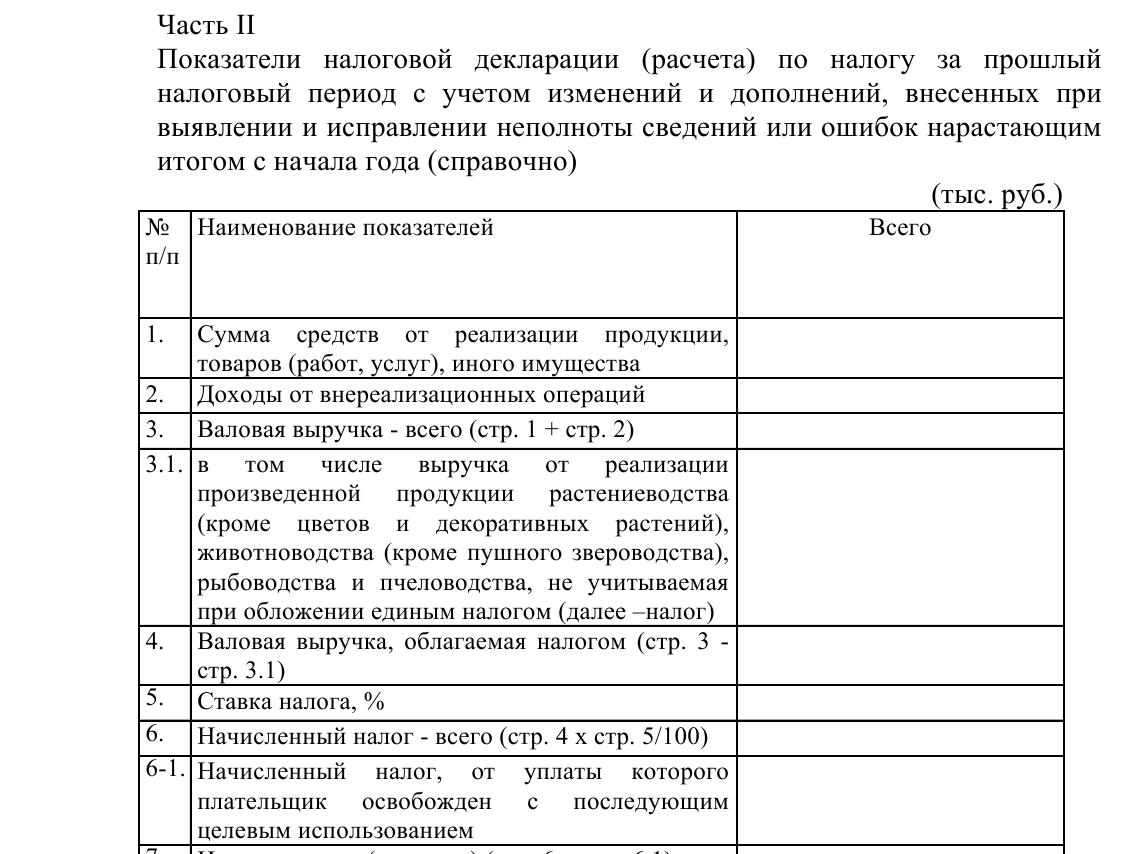
\includegraphics[scale=0.4]{pics/taxformrb}
  \caption{Фрагмент налоговой декларации}
  \label{pic:taxformrb}
\end{figure}


Налоговая декларация содержит различные данные о финансовой деятельности налогоплательщика. Процесс заполнения включает в себя процесс заполнения полей декларации. Существуют поля которые должны содержать информацию о финансовой деятельности налогоплательщика, поля которые представляют собой сумму каких-либо других полей декларации, поля, которые отображают отчетный период.

Заполнение налоговых деклараций на крупных предприятиях требует больших вычислений, которые связаны с учетом всей финансовой деятельности предприятия в отчетный период.
\section{Обзор существующих систем документооборота}
Рассмотрим существующие системы документооборота, которые позволяют автоматизировать процесс налоговой отчетности.
\subsection{Программный продукт 1C Бухгалтерия}
Программный продукт "1С:Бухгалтерия" — универсальная программа массового назначения для автоматизации бухгалтерского и налогового учета, включая подготовку обязательной (регламентированной) отчетности. Это готовое решение для ведения учета в организациях, осуществляющих любые виды коммерческой деятельности: оптовую и розничную торговлю, комиссионную торговлю (в том числе субкомиссию), оказание услуг, производство и т.д. Кроме того, с помощью ``1С:Бухгалтерии" могут вести учет индивидуальные предприниматели, применяющие упрощенную систему налогообложения или общий режим налогообложения.
\parБухгалтерский и налоговый учет реализованы в соответствии с действующим законодательством Российской Федерации. В состав конфигурации включен план счетов бухгалтерского учета, настроенный в соответствии с Приказом Минфина РФ "Об утверждении плана счетов бухгалтерского учета финансово-хозяйственной деятельности организаций и инструкции по его применению" от 31 октября 2000 г. № 94н.
\parМетодика бухгалтерского учета обеспечивает одновременную регистрацию каждой записи хозяйственной операции как по счетам бухгалтерского учета, так и по необходимым разрезам аналитического учета, количественного и валютного учета. Пользователи могут самостоятельно управлять методикой учета в рамках настройки учетной политики, создавать новые субсчета и разрезы аналитического учета.
\parПредметная область, автоматизируемая "1С:Бухгалтерией" изображена на рисунке~\ref{pic:1c_image1}.
\begin{figure}
  \centering
  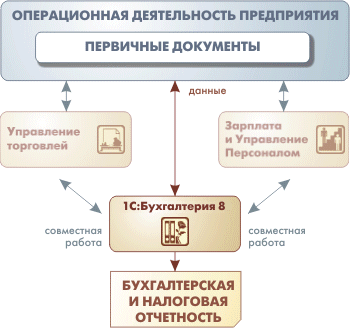
\includegraphics{pics/1c_image1}
  \caption{Предметная область, автоматизируемая ``1С:Бухгалтерией''}
  \label{pic:1c_image1}
\end{figure}
В подсистеме расчета заработной платы обеспечено формирование бумажной и электронной отчетности по налогам, связанным с заработной платой, в частности НДФЛ и ЕСН. Реализован персонифицированный учет взносов в Пенсионный фонд. Для расчета налогов и сборов и формирования налоговых деклараций используется регламентированная отчетность.
\begin{figure}
  \centering
  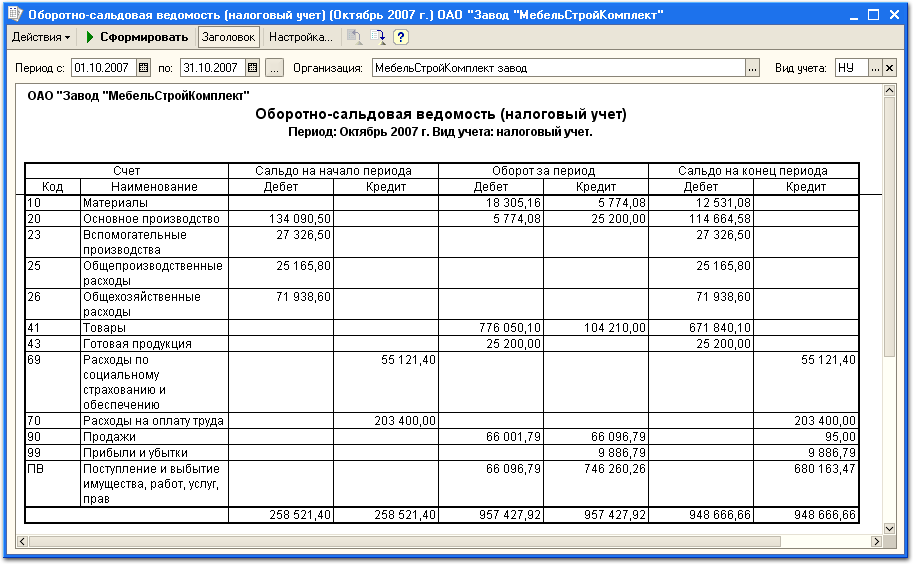
\includegraphics[scale=0.5]{pics/1c_image2}
  \caption{Окно для заполнения налогового декларации в системе 1С:Бухгалтерия}
  \label{pic:1c_image2}
\end{figure}
\subsection{Программный продукт Галактика ERP}
Автоматизированная система управления Галактика ERP (Enterprise Resource Planning) - это отечественная ERP-система для комплексной автоматизации бизнеса, основа комплекса Галактика Business Suite.
\parВозможности системы ERP позволяют в едином информационном пространстве оперативно решать главные управленческие задачи, обеспечить менеджеров различного уровня управления необходимой и достоверной информацией для принятия управленческих решений.
\parВ состав системы автоматизации управления предприятием Галактика ERP входят средства и для поддержки специальных управленческих задач:
\begin{itemize}
  \itemуправление техническим обслуживанием и ремонтами оборудования;
  \itemуправление качеством продукции;
  \itemуправление взаимоотношениями с клиентами;
  \itemуправление недвижимостью;
\end{itemize}
\parСистема состоит из нескольких функциональных блоков – контуров, каждый их которых решает комплекс задач: управление финансами, производством, логистикой, взаимоотношениями с клиентами и другие. Каждый контур состоит из нескольких модулей, нацеленных на выполнение более узких задач. Модульная структура Галактики ERP позволяет приобретать и использовать только те модули и контуры, которые необходимы конкретному предприятию. С развитием бизнеса и появлением новых управленческих задач, предприятие имеет возможность последовательно производить закупку необходимых компонент системы.
\parВ системе Галактика ERP реализована концепция компонентной модели: все единицы системы сформированы в компоненты, взаимодействующие между собой через специальные интерфейсы. Компоненты логически объединены в модули системы Галактика ERP. Наличие версий у компонентов позволяет перейти от обновления системы к обновлению отдельных компонентов.
\parСистема Галактика ERP поддерживает русский, белорусский, украинский и казахский языки.
\parВ состав системы Галактика ERP включены средства для централизованной настройки параметров системы, ее обновления, установки необходимых приложений. Это существенно повышает безопасность системы, улучшает защиту от несанкционированного доступа и значительно облегчает процесс ее администрирования.
Для автоматизированного учета налогов в системе Галактика ERP реализованы гибкие и универсальные механизмы, позволяющие оперативно ``подстраиваться'' под изменяющееся законодательство. Система дает возможность раздельного ведения бухгалтерского и налогового учета, формирования налоговых регистров и налоговой отчетности в соответствии с требованиями действующего налогового законодательства.
Принцип построения налогового учета в системе базируется на однократной регистрации первичных документов, формировании учетных записей от первичного документа с использованием настроенных типовых хозяйственных операций, использовании набора готовых деклараций и механизма настройки, а также создании пользовательских отчетных форм для расширения состава деклараций в соответствии с требованиями предприятия. Налоговая отчетность строится на данных первичных документов и сформированных по ним проводок. Для налогового учета можно использовать как параллельный план счетов, так и бухгалтерский план счетов, расширенный специально введенными для налогового учета синтетическими и аналитическими разрезами учета.
\parСредства системы Галактика ERP по ведению налогового учета сосредоточены не только в модуле Налоговый учет, но и в других модулях системы. В модуле Налоговый учет скомпонованы основные функциональные средства по документированию налогооблагаемой базы по налогу на прибыль. Он содержит специально разработанную систему интерактивных настраиваемых деклараций для формирования налоговых регистров. Функции для формирования регистров сгруппированы по типам операций. Каждый полученный в результате регистр отражает перечень показателей, на основе которых можно осуществить исчисление налоговой базы.
\subsection{Программный продукт Парус}
Программные продукты ``ПАРУС'' (ПП ``ПАРУС'') — предназначены для автоматизации деятельности коммерческих предприятий и бюджетных учреждений разного уровня. Среди линеек ПП ``ПАРУС'' есть и тиражные продукты и относящиеся к классу ERP-систем.
\parСистема строится на базе двухзвенной архитектуры клиент-сервер с использованием СУДБ Oracle(рисунок~\ref{pic:parus_pic1}).
\begin{figure}
  \centering
  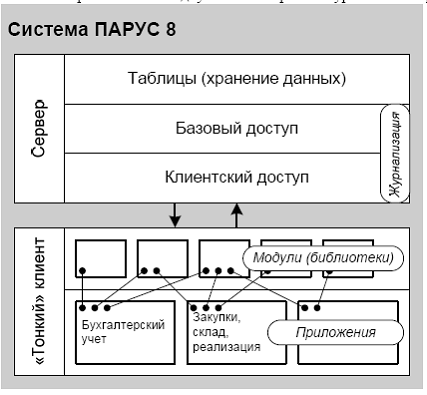
\includegraphics[scale=0.7]{pics/parus_img1}
  \caption{Двухзвенная архитектура системы ``ПАРУС''}
  \label{pic:parus_pic1}
\end{figure}
На сервере размещаются уровни:
\begin{itemize}
\itemхранения данных;
\itemбазового доступа: реализуются алгоритмы простейших бизнес-процедур;
\itemклиентского доступа: реализуются процедуры, составленные из одного или нескольких элементов базового доступа, – с поддержкой управления правами доступа пользователей и пользовательских настроек;
\end{itemize}
Возможные конфигурации построения:
\begin{itemize}
  \itemоднопользовательская;
  \itemлокальная сеть;
  \item WEB-решения;
  \itemтерминальный доступ;
\end{itemize}
Модуль ``Бухгалтерский учет'' предназначен для автоматизации ведения бухгалтерского учета в бюджетных учреждениях любого уровня. В модуле реализован документооборот всех участков бухгалтерского учета, которые ведут главные распорядители, распорядители и получатели бюджетных средств, в соответствии с положениями действующих нормативных документов.
В модуле реализованы учетные регистры для учета всех видов первичных документов и учетной информации, ведение которых предусмотрено нормативными документами, регулирующими ведение бухгалтерского учета. Модуль имеет интуитивно понятный интерфейс, все функциональные возможности сгруппированы по принципу принадлежности к участкам бухгалтерского учета. Благодаря широкому набору функциональных возможностей модуль позволяет полностью автоматизировать:
\begin{enumerate}
  \itemучет операций по санкционированию расходования бюджетных средств;
  \itemучет финансовых активов (операций с денежными средствами);
  \itemэлектронное взаимодействие с отделениями Федерального казначейства;
  \itemучет расчетов с поставщиками и подрядчиками;
  \itemучет нефинансовых активов;
\end{enumerate}
Упрощённая схема модуля ``Бухгалтерский учет'' и его взаимодействие с другими модулями представлено на рисунке~\ref{pic:parus_pic2}
\begin{figure}
  \centering
  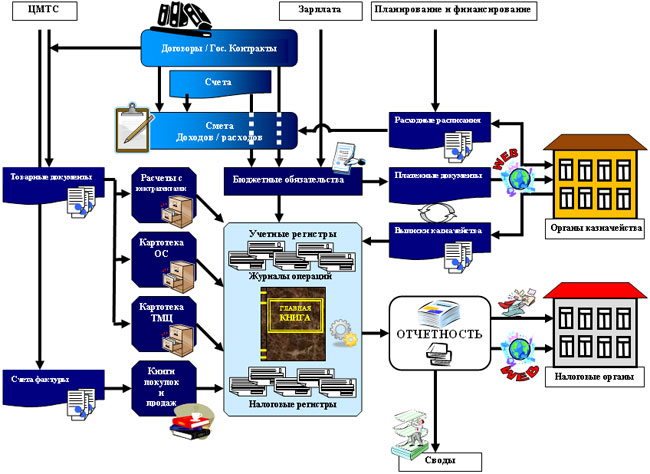
\includegraphics[scale=0.6]{pics/parus_img2}
  \caption{Упрощённая схема модуля ``Бухгалтерский учет''}
  \label{pic:parus_pic2}
\end{figure}
\subsection{Программный продукт Microsoft Dynamics NAV}
Программный продукт Microsoft Dynamics NAV — интегрированная система управления предприятием  класса ERP, поставляемая корпорацией Microsoft в новой линейке продуктов Microsoft Dynamics для среднего и малого бизнеса. В этой системе реализована следующая функциональность:
\begin{itemize}
  \itemуправление финансами;
  \itemбизнес-анализ;
  \itemуправление цепочками поставок;
  \itemуправление складом;
  \itemуправление отношениями с клиентами;
  \itemэлектронная коммерция;
  \itemпроизводство;
\end{itemize}
\parФинансовый контур системы Microsoft Dynamics NAV полностью интегрирован с функциональностью управления складом и производством, а также с блоками расчетов с клиентами и поставщиками, учета основных средств, заработной платы. Это позволяет автоматически и в режиме реального времени отражать на финансовых счетах главной книги себестоимость товаров, произведенной продукции и оказанных услуг, а также скидки, издержки, накладные расходы, начисление НДС и прочие данные. Уникальная технология индексного суммирования позволяет мгновенно обновлять итоговые суммы после проведения транзакции любой сложности. Благодаря этому можно в режиме реального времени получить показатели за любой период и с любым количеством установленных фильтров.
\par Microsoft Dynamics NAV позволяет автоматически создавать корпоративную отчетность любой степени детализации и сложности. Отчетность формируется независимо от планов счетов, количества анализируемых показателей, валюты и продолжительности учетных периодов фирм-филиалов. Многовалютность системы позволяет вести баланс в рублях и в дополнительной отчетной валюте. При этом полностью сохраняется история операций с точки зрения оригинальной валюты.
\par Microsoft Dynamics NAV отличается мощными средствами трассировки и контроля источников происхождения любой операции, что делает прозрачными и доступными для понимания самые сложные транзакции. В системе автоматически формируются учетные финансовые регистры. Уникальная функция ``Навигатор'' позволяет на основании даты и номера документа выявить все взаимосвязанные операции и документы, выяснить дату построения транзакции и идентифицировать создавшего ее пользователя.
\par Microsoft Dynamics NAV отличается гибкостью настройки бизнес-правил и процедур учета, возможностями модификации стандартных форм и деклараций. Это позволяет вам легко и быстро адаптировать систему к любым изменениям в бизнесе, самостоятельно расширяя детализацию аналитики и тем самым создавая ваше собственное информационное решение.
\par Microsoft Dynamics NAV содержит средства бюджетирования, планирования и мониторинга бюджетов. Бюджетная система компании может включать любое количество бюджетов с разной степенью детализации – от подразделений до сводных бюджетов всего холдинга. Аналитические измерения позволяют создавать бюджеты по индивидуальным статьям затрат и доходов. Система матричных форм бюджетов предназначена как для мониторинга деятельности отдельных подразделений компании, так и для сравнения с показателями любых предыдущих периодов.
\parДля дополнительного удобства и гибкости работы с бюджетами в Microsoft Dynamics NAV предусмотрена интеграция с Microsoft Office Excel, которая позволяет импортировать и экспортировать бюджетные показатели.
Межфирменный учет упрощает и оптимизирует бизнес-процессы и транзакции, проводимые между всеми структурными единицами бизнеса, имеющими отдельный баланс. Внедрение этого модуля позволяет эффективно управлять дочерними и внутренними организациями-партнерами, филиалами и аффилированными компаниями, в том числе находящимися в других странах.
\parРабочая среда Microsoft Dynamics NAV позволяет рассылать документы о продажах и покупках и распространять операции финансового журнала на все подчиненные офисы, коммерческие отделы или дочерние компании, что упрощает документооборот и снижает трудозатраты. Информация о межфирменной транзакции вводится в соответствующие документы только один раз.
\parПользователи полностью контролируют все документы, связанные с транзакциями. Например, они могут отклонить присланный им документ и таким образом аннулировать неверные проводки. Осуществляя закупку у компании-партнера или дочерней фирмы, они могут корректировать заказ, пока не начнется отгрузка товара.
\parДля формирования бухгалтерской и налоговой отчетности реализован механизм, позволяющий заполнять отчетные формы на основании данных по финансовым счетам, операциям с НДС и заработной плате сотрудников. При этом пользователь может самостоятельно, не прибегая к помощи специалиста, управлять механизмом формирования отчетности, динамически изменяя алгоритм расчета строк документов с учетом текущего изменения плана счетов и аналитики.
\parС помощью механизма регламентной отчетности можно выгружать данные из регламентных деклараций Microsoft Dynamics NAV в шаблоны файлов Microsoft Office Excel. Интеграция с Microsoft Office Excel позволяет хранить в базе данных Microsoft Dynamics NAV шаблоны выходных форм и экспортировать итоги вычислений в определенные ячейки файла-шаблона, что существенно повышает гибкость работы с результирующими формами и обеспечивает поддержку актуальности бухгалтерских форм.
\parВ декларациих активно используются разнообразные фильтры и переменные параметры. В частности, в подмодуле ``Финансовые операции'' представлен перечень внутренней отчетности, необходимой в работе бухгалтера. Это журналы-ордера, оборотные ведомости, ``шахматки'', бухгалтерские карточки счетов, поставщиков, клиентов и банков, анализ счета и т.д. Помимо бухгалтерских деклараций внутреннего пользования Microsoft Dynamics NAV содержит большой набор унифицированных форм документов по учету основных средств, кассовых и банковских операций, складские, товарно-отгрузочные документы и т.д. При необходимости любой отчет может быть модифицирован и адаптирован применительно к специфике деятельности предприятия.
\parОдин из основных участков ведения учета – учет кассовых и банковских операций. В Microsoft Dynamics NAV реализован весь спектр кассовых операций. Подмодуль ``Денежные средства'' модуля ``Финансы'' позволяет заносить и учитывать приходные и расходные ордеры на клиентов, поставщиков и подотчетных лиц, на банковские счета и напрямую на финансовый счет. Реализованы все декларации, необходимые для ведения кассовых операций:
\begin{itemize}
  \itemприходный кассовый ордер;
  \itemрасходный кассовый ордер;
  \itemкассовая книга;
  \itemжурнал регистрации приходных и расходных ордеров;
\end{itemize}
\parКаждая компания может вести неограниченное количество расчетных счетов в любой валюте. Система хранит полную историю проведения платежей, включая формирование платежного документа, внесение изменений в документ, отмену документа, повторное создание документа и т.д.
\begin{figure}
  \centering
  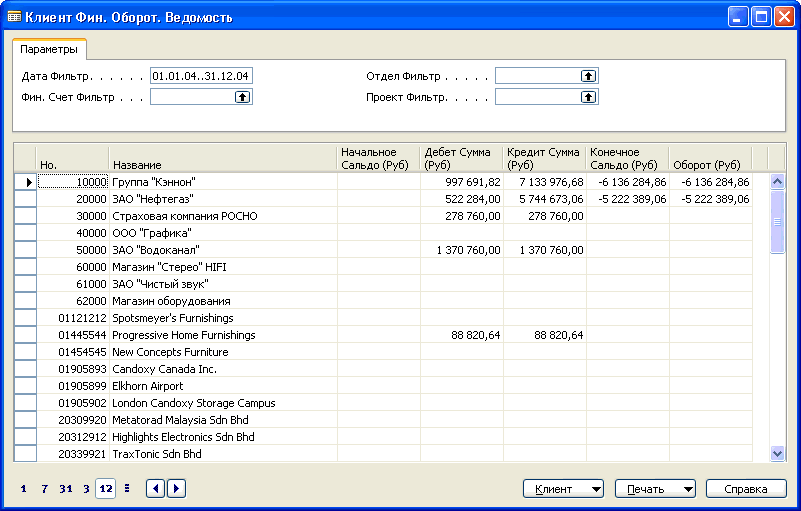
\includegraphics[scale=0.50]{pics/navision_img1}
  \caption{Оборотная ведомость в разрезе клиентов}
  \label{pic:navision_pic1}
\end{figure}

\subsection{Сравнение систем документооборота}
Проведем сравнение рассмотренных систем документооборота. Сравнение будем производить по следующим критериям:
\begin{itemize}
  \itemТип - тип системы документооборота, который показывает предметную область в управлении предприятием (которая может включать в себя не только финансовую деятельность) которую автоматизирует система;
  \itemОС - поддерживаемые операционные системы;
  \itemСтруктура - структура приложения, которую представляет собой рассматриваемая система;
  \itemБаза данных - тип базы данных, которая используется для хранения информации;
  \itemЛицензия - лицензия, под которой распространяется система;
\end{itemize}
Результаты сравнения приведены в таблицах~\ref{tabl:analys_1} и ~\ref{tabl:analys_2}
\begin{table}
  \centering
  \caption{Результат сравнения систем документооборота(Начало)}
  \label{tabl:analys_1}
\begin{tabular}{|m{3.2cm}|m{3cm}|m{2cm}|m{2.5cm}|m{4cm}|}
  \hline
  \bfseries{Название системы} &
  \bfseries{Тип} &
  \bfseries{ОС} &
  \bfseries{Структура} &
  \bfseries{База Данных}\\
  \hline
  1C Бухгалтерия & Система бухгалтерского учета & Windows, GNU Linux & Standalone, Web & 1CD(собственный формат), Microsoft SQL Server, DBF\\
  \hline
  Галлактика ERP & Система планирования ресурсов предприятия & Windows  & Standalone  & PervasiveSQL, Microsoft SQL Server, Oracle\\
  \hline
  Парус & Система планирования ресурсов предприятия & Windows & Standalone, Web & Oracle\\
  \hline
  Microsoft Dynamic NAV & Система планирования ресурсов предприятия & Windows & Standalone, Web & Microsoft SQL Server\\
  \hline
\end{tabular}
\end{table}
\begin{table}
  \centering
  \caption{Результат сравнения систем документооборота(Продолжение)}
  \label{tabl:analys_2}
\begin{tabular}{|m{6cm}|m{4cm}|}
  \hline
  \bfseries{Название системы} &
  \bfseries{Лицензия}\\
  \hline
  1C Бухгалтерия & Коммерческая\\
  \hline
  Галлактика ERP & Коммерческая\\
  \hline
  Парус & Коммерческая\\
  \hline
  Microsoft Dynamic NAV & Коммерческая\\
  \hline
\end{tabular}
\end{table}

\chapter{Проектирование системы создания и управления электронными налоговыми декларациями}
Разрабатываемая система должна решать следующие задачи:
\begin{itemize}
  \itemавтоматизация заполнения налоговых деклараций;
  \itemпредоставление процесса утверждения документа;
  \itemотправка заполненных деклараций в налоговую инспекцию;
\end{itemize}
\section{Требования, предъявляемые к системе}
В качестве исходных данных были предъявлены следующие требования к разрабатываемой системе:
\begin{enumerate}
  \itemСистема должна обеспечить разграничение прав. Система должна поддерживать работу пользователей, каждый пользователь может иметь свои настройки. Группа пользователей объединяется в домен, в каждом домене есть администратор, который может добавлять, удалять пользователей, либо изменять настройки каждого пользователя из домена.
  \itemСистема должна предоставлять web интерфейс. Для работы с системой пользователь должен иметь возможность использовать web-интерфейс, что позволяет использовать систему практически из любого окружение, для доступа к системе нужен только веб-браузер.
  \itemДля хранения данных должна использоваться реляционная база данных. Данные о заполненных декларациих должны храниться в реляционной базе данных.
  \itemТребуется обеспечить возможность добавление новых деклараций и изменения существующих. декларации могут изменяться (добавляться, удаляться, изменяться содержимое) в каждом налоговом году, для этого необходимо предоставить простой способ для достижения этой цели.
%  \itemТребуется обеспечить экспорт заполненых деклараций в формат Adobe Pdf. После того как декларации заполнены необходимо обеспечить их экспорт в формате Adobe Pdf для последующей печати. Adobe Pdf файл для каждой декларации должен генерироваться по заданному шаблону.
%  \itemСистема должна предоставлять возможность отправки деклараций в налоговую инспекцию. После того как декларации заполнены, их можно отправить в налоговую инспекцию в виде документа, который генерируется на основе заполненных деклараций, согласно используемому в налоговой службе формату.
  \itemТребуется предоставить возможность изменения правил подсчета для ячеек деклараций. Ячейки, которые считаются по формулам, либо по каким-то другим правилам могут быть переписаны произвольным значением, которые задаст пользователь.
\end{enumerate}

\section{Анализ требований}
Проведем анализ предъявленных требований:
\begin{enumerate}
  \itemТребуется ввести сущность Пользователь и Домен. Все сущности, которые будут создаваться пользователями в системе не будут доступны для пользователей из других доменов, так же можно ограничить доступ к создаваемым сущностям для пользователей одного домена. Пользователь будет однозначно идентифицироваться доменом, именем. Для входа в систему пользователю необходимо ввести пароль.
  \itemСистема будет представлять собой клиент-серверное приложение, в котором клиентом будет выступать браузер(иногда называется ``тонким клиентом''), а сервером - веб-сервер. Логика веб-приложения распределена между сервером и клиентом, хранение данных будет осуществляться на сервере, обмен данными будет происходить по сети. Возможность обновления и поддержки веб-приложений без установки дополнительного программного обеспечения у клиента является одной из ключевых причин популярности веб приложений.
  \itemВся информация о сущностях, созданных пользователями будет храниться в реляционной базе данных. Реляционная база данных - база данных, основанная на реляционной модели данных. Реляционная модель данных основана на математическом понятии отношение (relation). Для работы с реляционными базами данных применяются реляционные Системы Управления Базами Данных (СУБД). Наиболее известные реляционные СУБД: MySQL, Oracle, Postgres. Для создания, модификации и управления данными обычно используется язык Structured Query Language (SQL).
  \itemДля обеспечения добавления новых деклараций и изменения старых необходимо выделить структуры для представления деклараций и физическое представление этих структур. Для представления деклараций будет использоваться язык XML, каждый отчет будет описан с использованием данного языка. XML (eXtensible Markup Language) — рекомендованный Консорциумом Всемирной паутины язык разметки, фактически представляющий собой свод общих синтаксических правил. XML — текстовый формат, предназначенный для хранения структурированных данных , для обмена информацией между программами, а также для создания на его основе более специализированных языков разметки (например, XHTML), иногда называемых словарями.
\begin{figure}
  \centering
  \begin{small}
    \begin{verbatim}
      <instructions>
         <step>Смешать</step>
         <step>Закрыть</step>
         <step>Замесить</step>
      </instructions>
    \end{verbatim}
  \end{small}
  \caption{Пример XML документа}
  \label{pic:xml_sample}
\end{figure}
%  \item PDF (Portable Document Format) — кроссплатформенный формат электронных документов, созданный фирмой Adobe Systems с использованием ряда возможностей языка PostScript. В первую очередь предназначен для представления в электронном виде полиграфической продукции, значительное количество современного профессионального печатного оборудования мо%жет обрабатывать PDF непосредственно. Для создания PDF документов в языке Java можно ис%пользовать библиотеку iText.
  \item Для выполнения данного требования необходимо выделить сущность, которая будет представлять тип подсчета для ячейки.
\end{enumerate}

\section{Объектная модель системы}
Для проектирования системы будем использовать объектный подход.

Выделим объекты системы и определим отношения между ними, отразим результат на диаграмме сущность-связь, представленной на рисунке~\ref{pic:er_diagram}. Для предоставления возможности разграничения доступа будем использовать объекты ``Домен'' и ``Пользователь''. ``Домен'' объединяет какую-то группу ``Пользователей'', каждый пользователь в соответствии со своими правами доступа сможет или не сможет использовать объекты, которые были созданы другими ``Пользователями'' в данном ``Домене''. Объекты из одного ``Домена'' не доступны ``Пользователям'' из другого ``Домена''. Другим ключевым объектом в системе является ``Компания'', который инкапсулирует свойства компании, сотрудники которой будут использовать разрабатываемую систему. ``Компания'' содержит ``Налоговые формы'' - сущность, которая представляет собой совокупность документов, требуемых для налоговой отчетности (``Деклараций''). Сущность ``Декларация'' является представлением финансового декларации.''Декларация'' состоит из ``Ячеек'' - полей, которые содержат информацию, которая требуется согласно форме, которую представляет декларация. Каждая ``Ячейка'' имеет свое состояние(``Состояние ячейки'') c атрибутами ``Значение'' и ``Тип ячейки'', который показывает правила подсчета для конкретного типа, рассмотрим несколько возможных типов:
\begin{itemize}
  \itemФормула: ``Тип ячейки'' будет содержать формулу,например:\{A20\}+\{A40\}-\{A50\}*\{A60\} . A20, A40, A50 и A60 являются названием других ячеек, значения которых подставляются для подсчета формулы
  \itemЗначение определенное пользователем: ``Тип ячейки'' будет указывать на то, что в качестве значения требуется взять значение атрибута ``Значение'' объекта ``Состояние ячейки'', это означает, что значение должен задать пользователь
\end{itemize}
Ячейка так же имеет атрибут ``Тип данных'', который показывает какой тип данных имеет атрибут ``Значение'' ``Состояния ячейки''. ``Состояние ячейки'' имеет ``Текущий тип'', который является одним из возможных ``Типов ячейки''. ``Типы ячейки'' представляют собой набор допустимых типов, которые будут использоваться для подсчета данной ячейки, опираясь на пример, который содержит возможные типы, можно выделить следующие множества ``Типов ячейки''.
Отдельно выделим объект ``Состояние декларации'' который будет содержать данные, которые будут представлять состояние декларации - состояния всех ячеек декларации. Данное решение было принято для отделения статических данных декларации от динамических. Декларация со свойствами ячеек: имя, допустимые типы ячеек, представляет собой статические данные, которые будут меняться при необходимости изменить структуру декларации (например добавление новой ячейки, изменение имени ячейки, добавление либо удаление возможного типа ячейки), а такие свойства как ``Текущий тип'', ``Значение'' будут меняться при создании, либо редактировании декларации для конкретной ``Налоговой формы''. ``Объект загрузки состояния'' отвечает за загрузку ``Состояния декларации'', ``Объект сохранения состояния'' отвечает за сохранение состояния, согласно требованиям, хранение данных должно осуществляться в СУБД.
Для загрузки статических данных ``Декларации'' будет использоваться объект ``Загрузчик декларации'', который будет загружать данные для декларации и использовать ``Загрузчик ячейки'' для загрузки данных для каждой ячейки. В соответствии с анализом требования о предоставлении возможности добавления новых деклараций и изменения старых, было решено для хранения ``Деклараций'' использовать формат XML, соответственно ``Загрузчик декларации'' будет выполнять загрузку свойств декларации, а за обработку частей описания ``Декларации'' в формате XML, которые соответствуют ячейкам, будет отвечать ``Загрузчик ячейки''.
Объект ``Интерпретатор декларации'' будет совершать подсчет ``Декларации'', в свою очередь, данный объект будет использовать ``Интерпретатор ячейки'' для подсчета каждой ``Ячейки'' для декларации. Результатом подсчета ``Ячейки'' будет являться значение атрибута ``Значение'' объекта ``Состояние ячейки''. ``Интерпретатор ячейки'' будет производить подсчет ячейки в зависимости от ``Текущего типа'' ``Состояния ячейки''.
''ОтображениеДекларации'' отвечает за представление декларации пользователю. Это может быть, как декларация на веб-странице, так и декларация в каком-либо кросс-платформенном формате, например PDF или CSV.
\begin{figure}
  \centering
  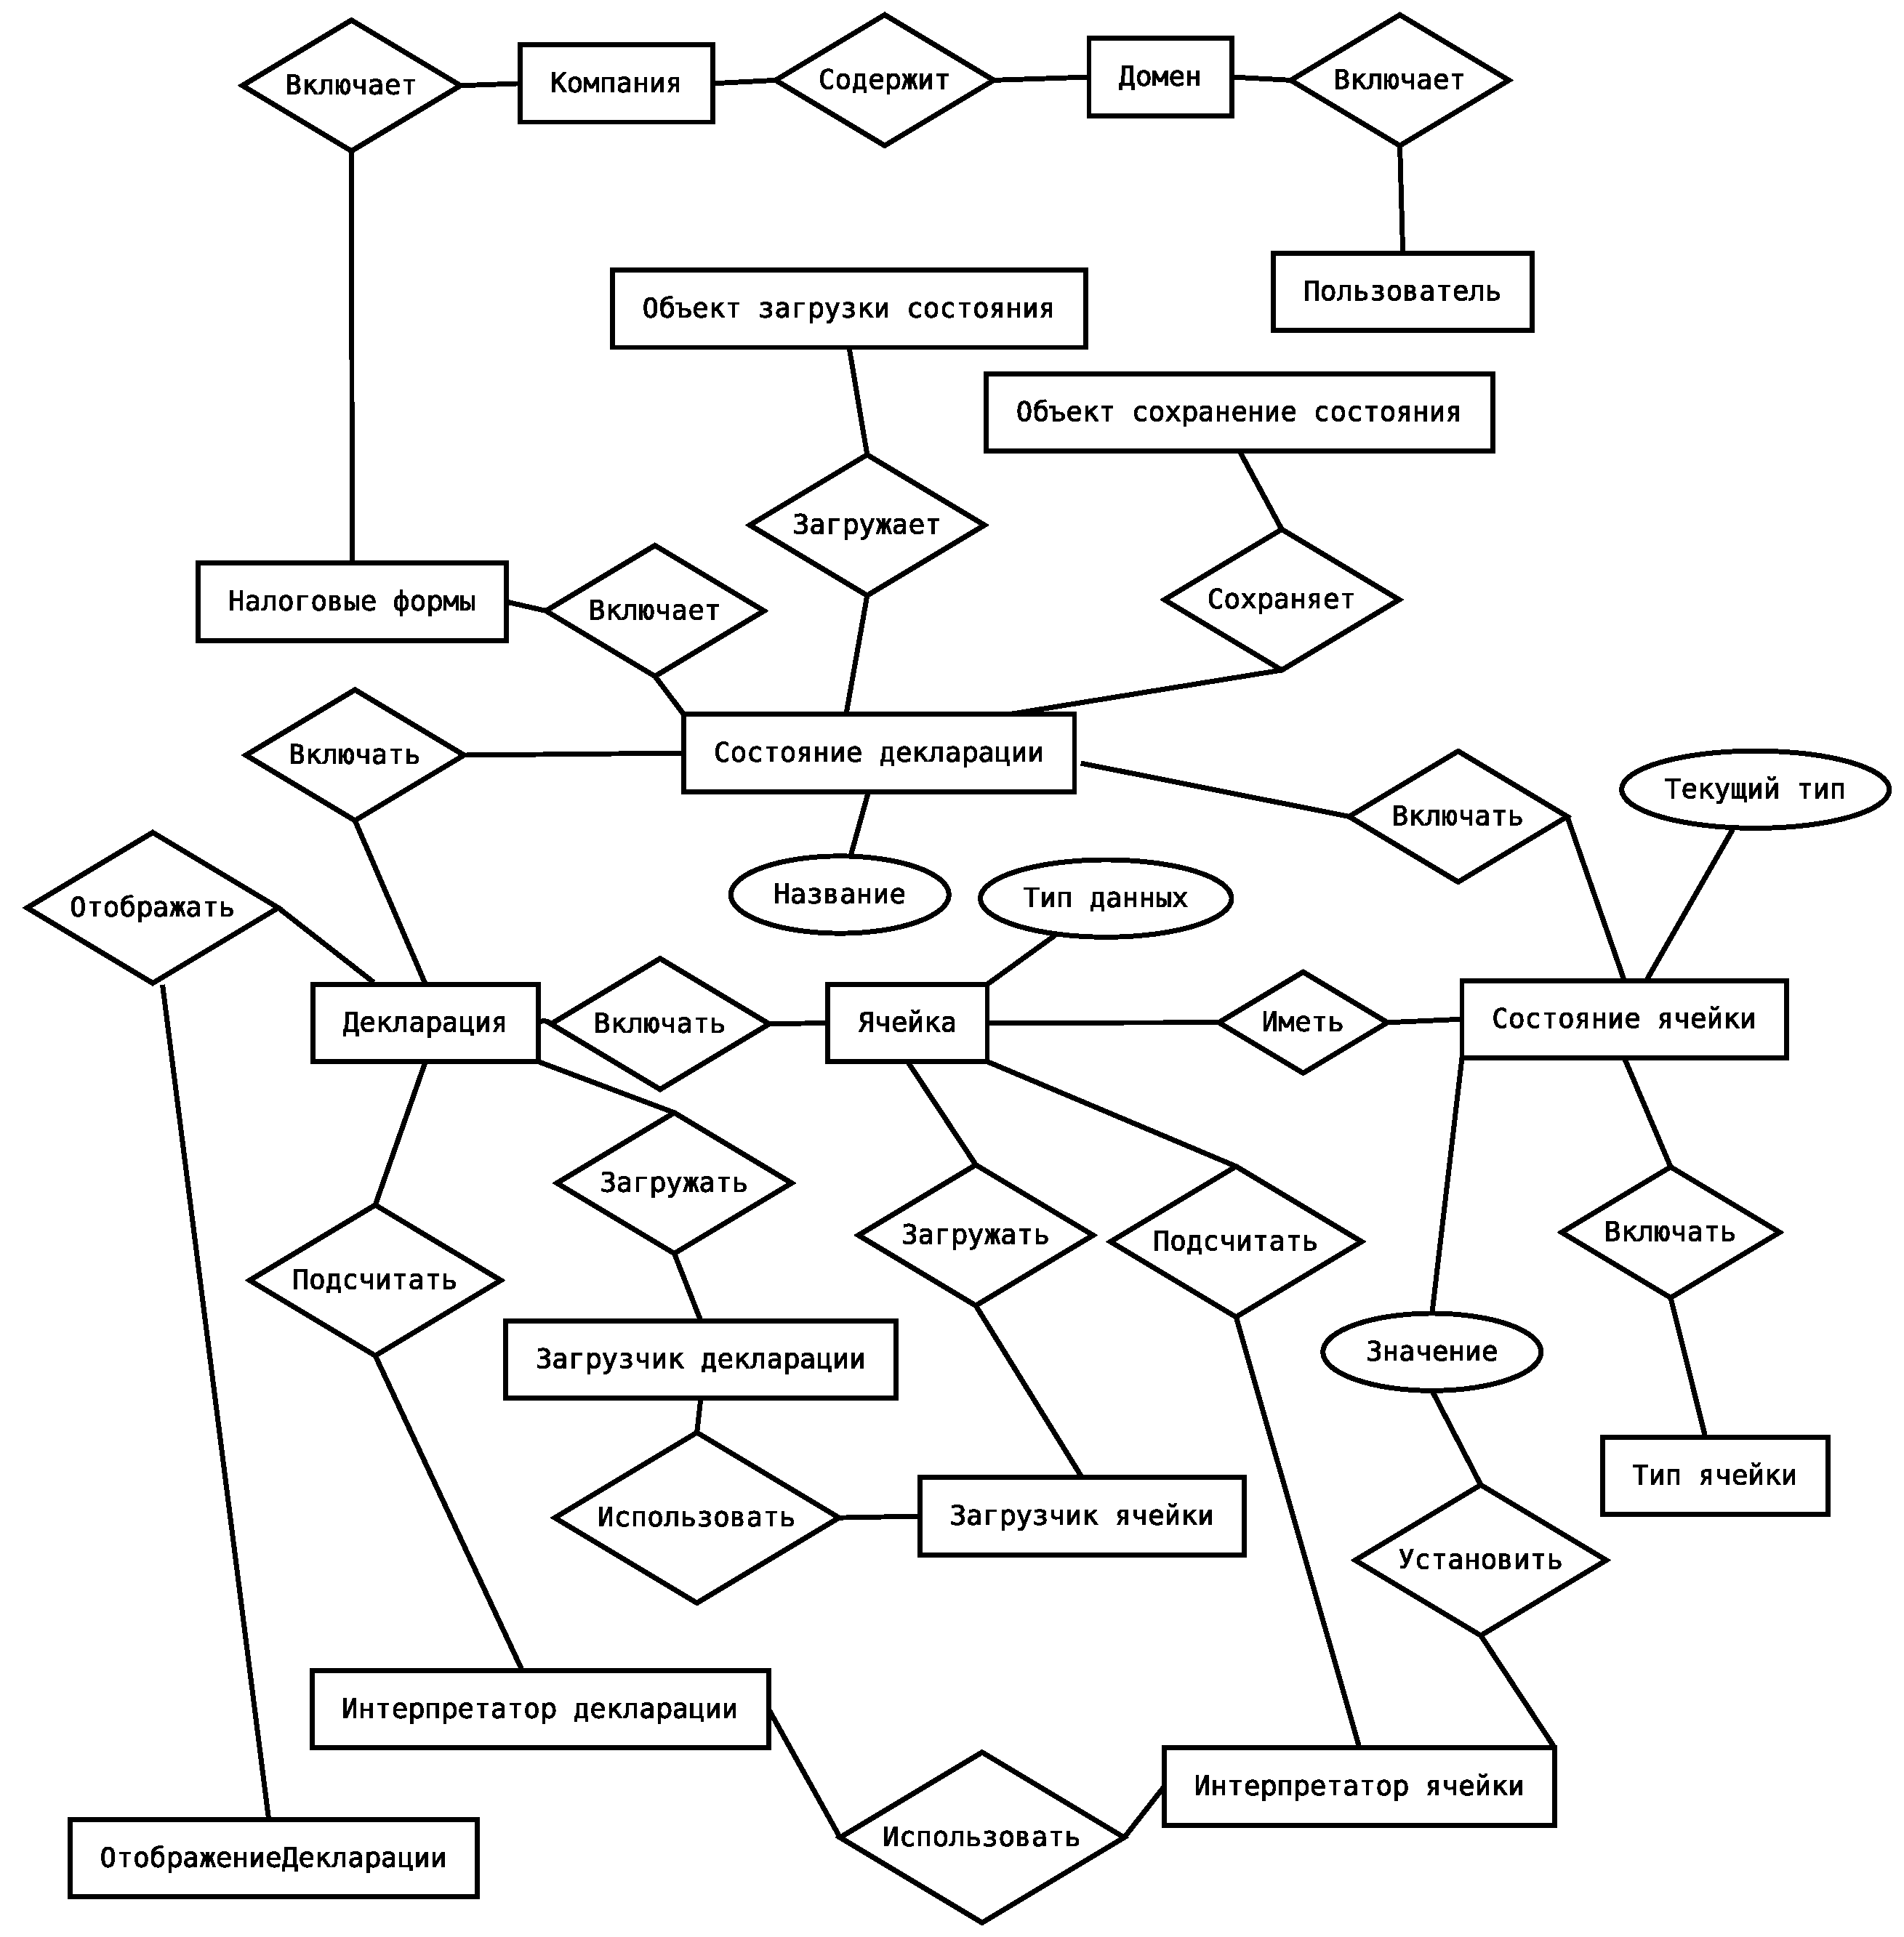
\includegraphics[scale=0.4]{uml/entity}
  \caption{Диаграмма сущность-связь}
  \label{pic:er_diagram}
\end{figure}
Так как значения в ячейках деклараций могут содержать значение, которое определено пользователем приложения, либо значение, которое представляет некое алгебраическое выражение, которое для подсчета использует значения других ячеек, выделим следующие ``ТипыЯчеек'':
\begin{itemize}
  \item ``Формула''
  \item ``Редактируемая''
\end{itemize}


На диаграмме вариантов использования отразим возможные варианты действий пользователя системы при работе с декларацией (риcунок~\ref{pic:use_case_1}).


Для того чтобы произвести подсчет декларации пользователь должен его открыть. После открытия декларации пользователь может производить действия непосредственно с ячейками. Пользователь может пересчитать значение ячейки, может изменить параметры типа ячейки, например, если ячейка в данный момент считается как сумма/разность дебета либо кредита интервала банковских счетов, то пользователь может изменить данный интервал. Пользователь может изменить тип ячейки, если, например ячейка в данный момент считается как формула и в возможных типах ячейки присутствует возможность ввода значения пользователем, то пользователь может ввести свое значение, вместо значения, которое было подсчитано по формуле.
\begin{figure}
  \centering
  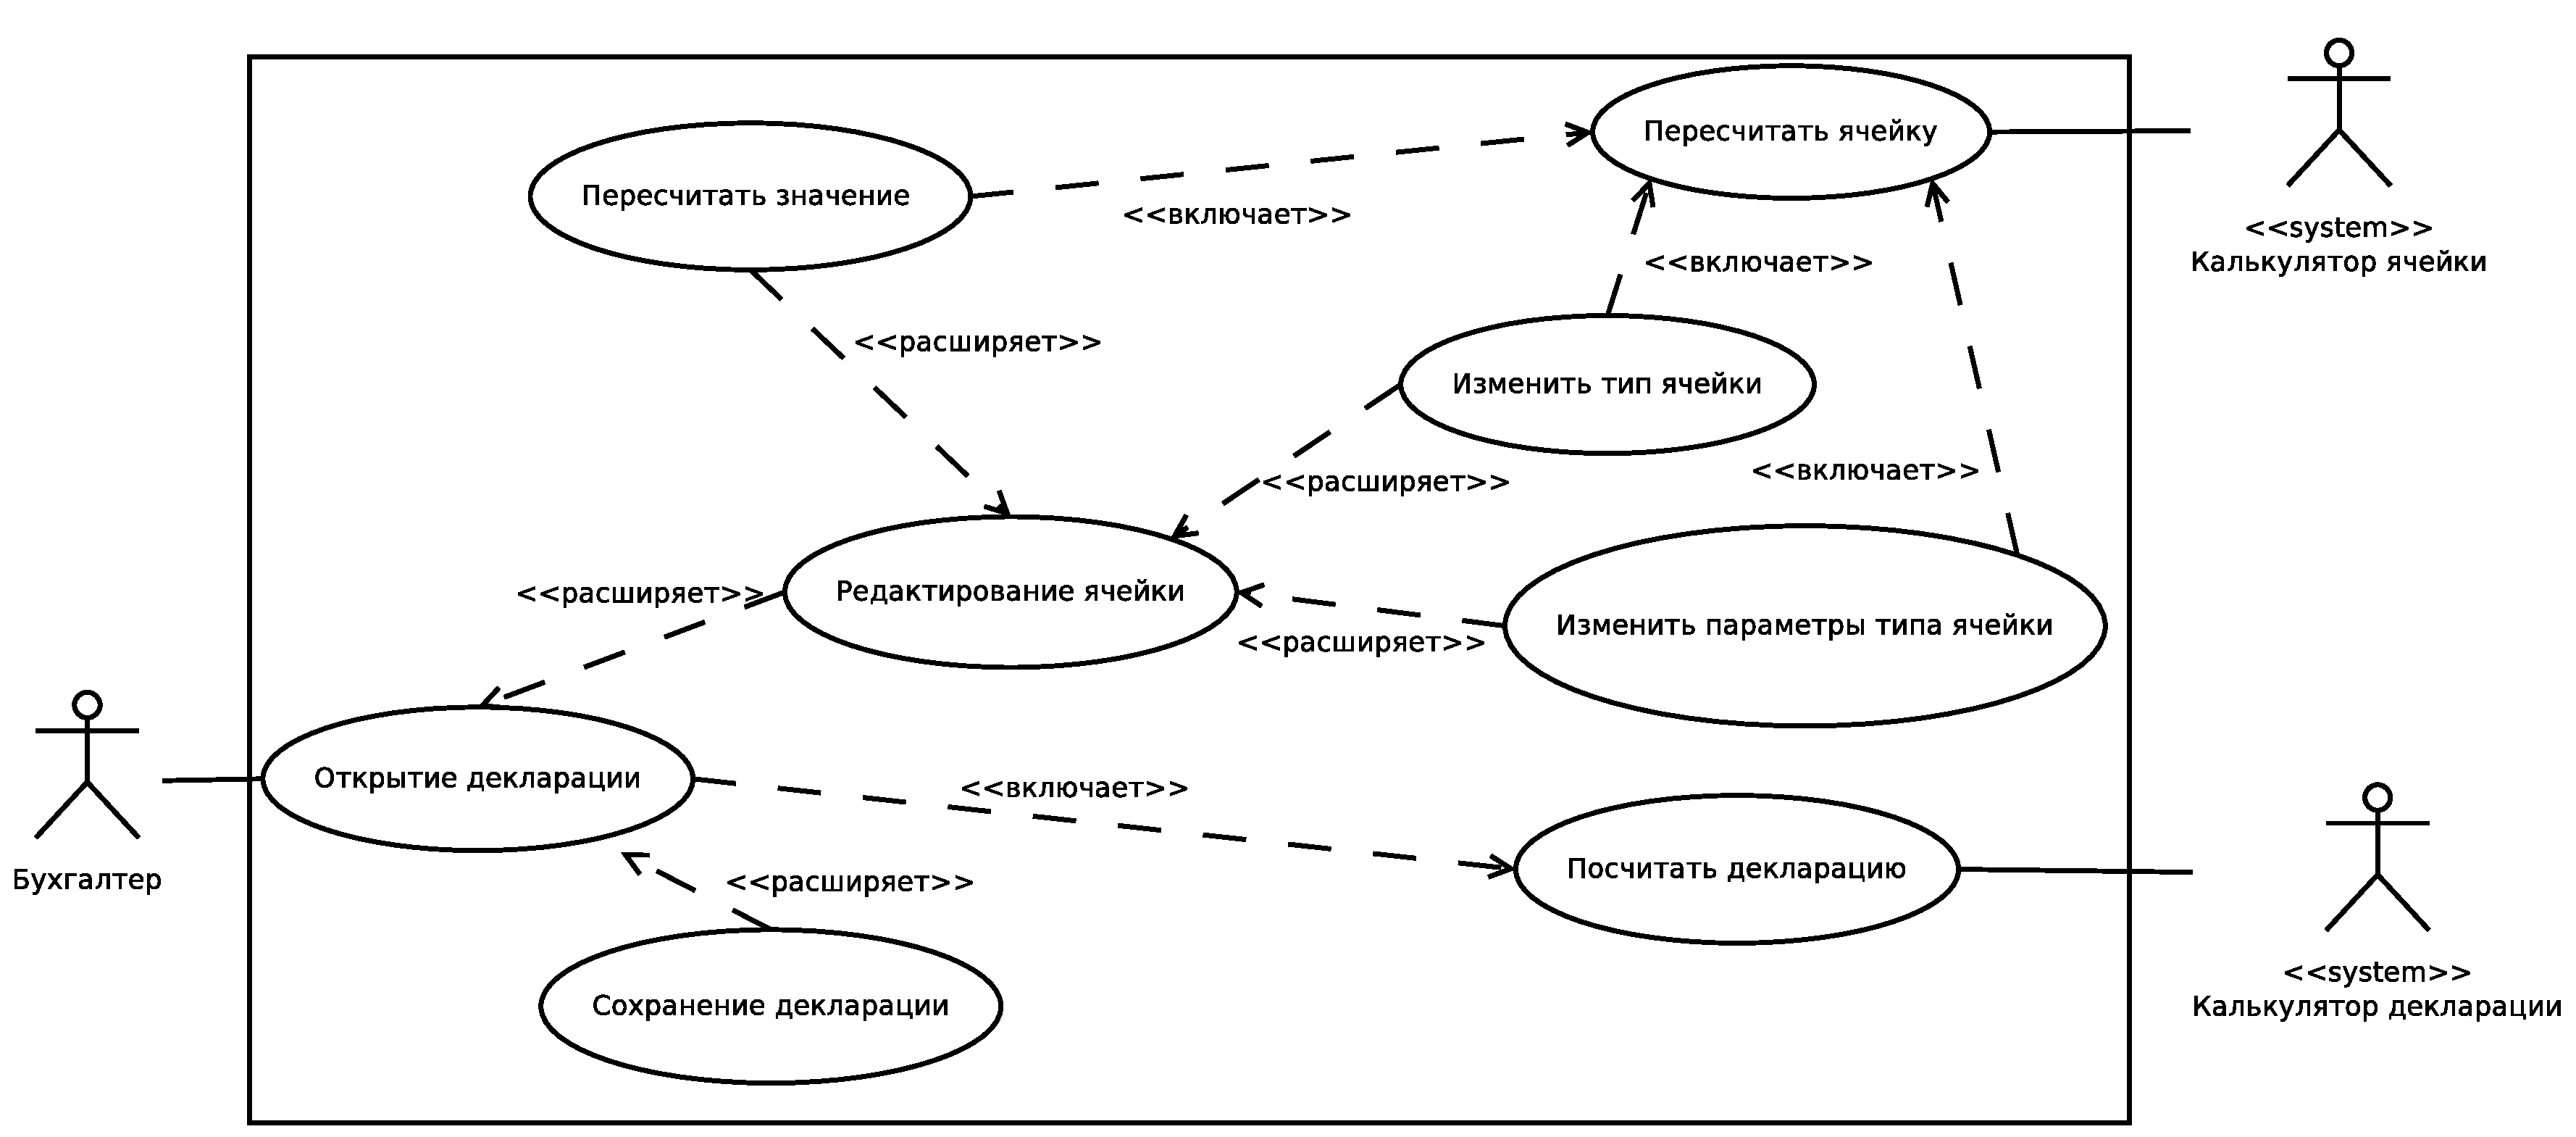
\includegraphics[scale=0.4]{uml/usecase_1}
  \caption{Диаграмма вариантов использования для декларации}
  \label{pic:use_case_1}
\end{figure}


На рисунке~\ref{pic:classes_1} представлена диаграмма классов. ``Сервис Декларации'' предоставляет методы для создания декларации (``загрузитьДекларация'') и сохранения его состояния (``сохранитьДекларация''). ``Менеджер Декларации'' содержит методы для управления состоянием декларации, таким как пересчет ячеек и изменения текущего типа ячейки. Метод ``изменитьТипЯчейки'' принимает ``СостояниеЯчейки'', в зависимости от параметра ``текущийТип'' пересчитывет данную ячейку и ячейки, которые зависят от данной. ``МенеджерыДеклараций'' содержит экзепляры классов ``Менеджер Декларации'', предоставляет методы для загрузки ``Менеджера Декларации'' по названию декларации и номеру ``Налоговых Форм''. Такое поведение необходимо в веб-приложении, так как протокол HTTP не поддерживает состояния, это значит, что после того как браузер послал запрос на сервер, физическое соединение закрывается. Казалось бы, что этот вопрос можно решить сохранением состояния декларации после каждого запроса на изменение состояние ячейки, но у такого подхода имеется ряд недостатков,основным является то, что при большом количестве пользователей нагрузка на СУБД возрастет и это отражается на производительности системы. В данном случае, при создании декларации, будет создаваться ``Менеджер Деклараций'', который будет оперировать декларацией, однозначно определенным по имени и номеру ``Налоговых Форм'', и сохраняться в памяти, откуда его можно будет получить при последующем обращении пользователя при помощи ``МенеджеровДеклараций''. ``ОбъектДоступаКСостояниюДекларации'' является абстрактным классом, реализация которого должна предоставлять реализацию методов ``загрузить'' и ``сохранить'' которые соответственно отвечают за загрузку и сохранение ``Состояния Декларации'' в базе данных. Абстрактный класс ``Фабрика декларации'' содержит метод ``создать'' который отвечает за создание ``Декларации'' по имени, реализация данного класса должна инкапсулировать загрузку ``Декларации'' из физического представления (XML). Классы ``КонтроллерДекларации'' и ``КонтроллерСостоянияДекларации'' обрабатывают события, которые были получены от пользователя посредством интерфейса пользователя (Web).
\begin{sidewaysfigure}
  \centering
  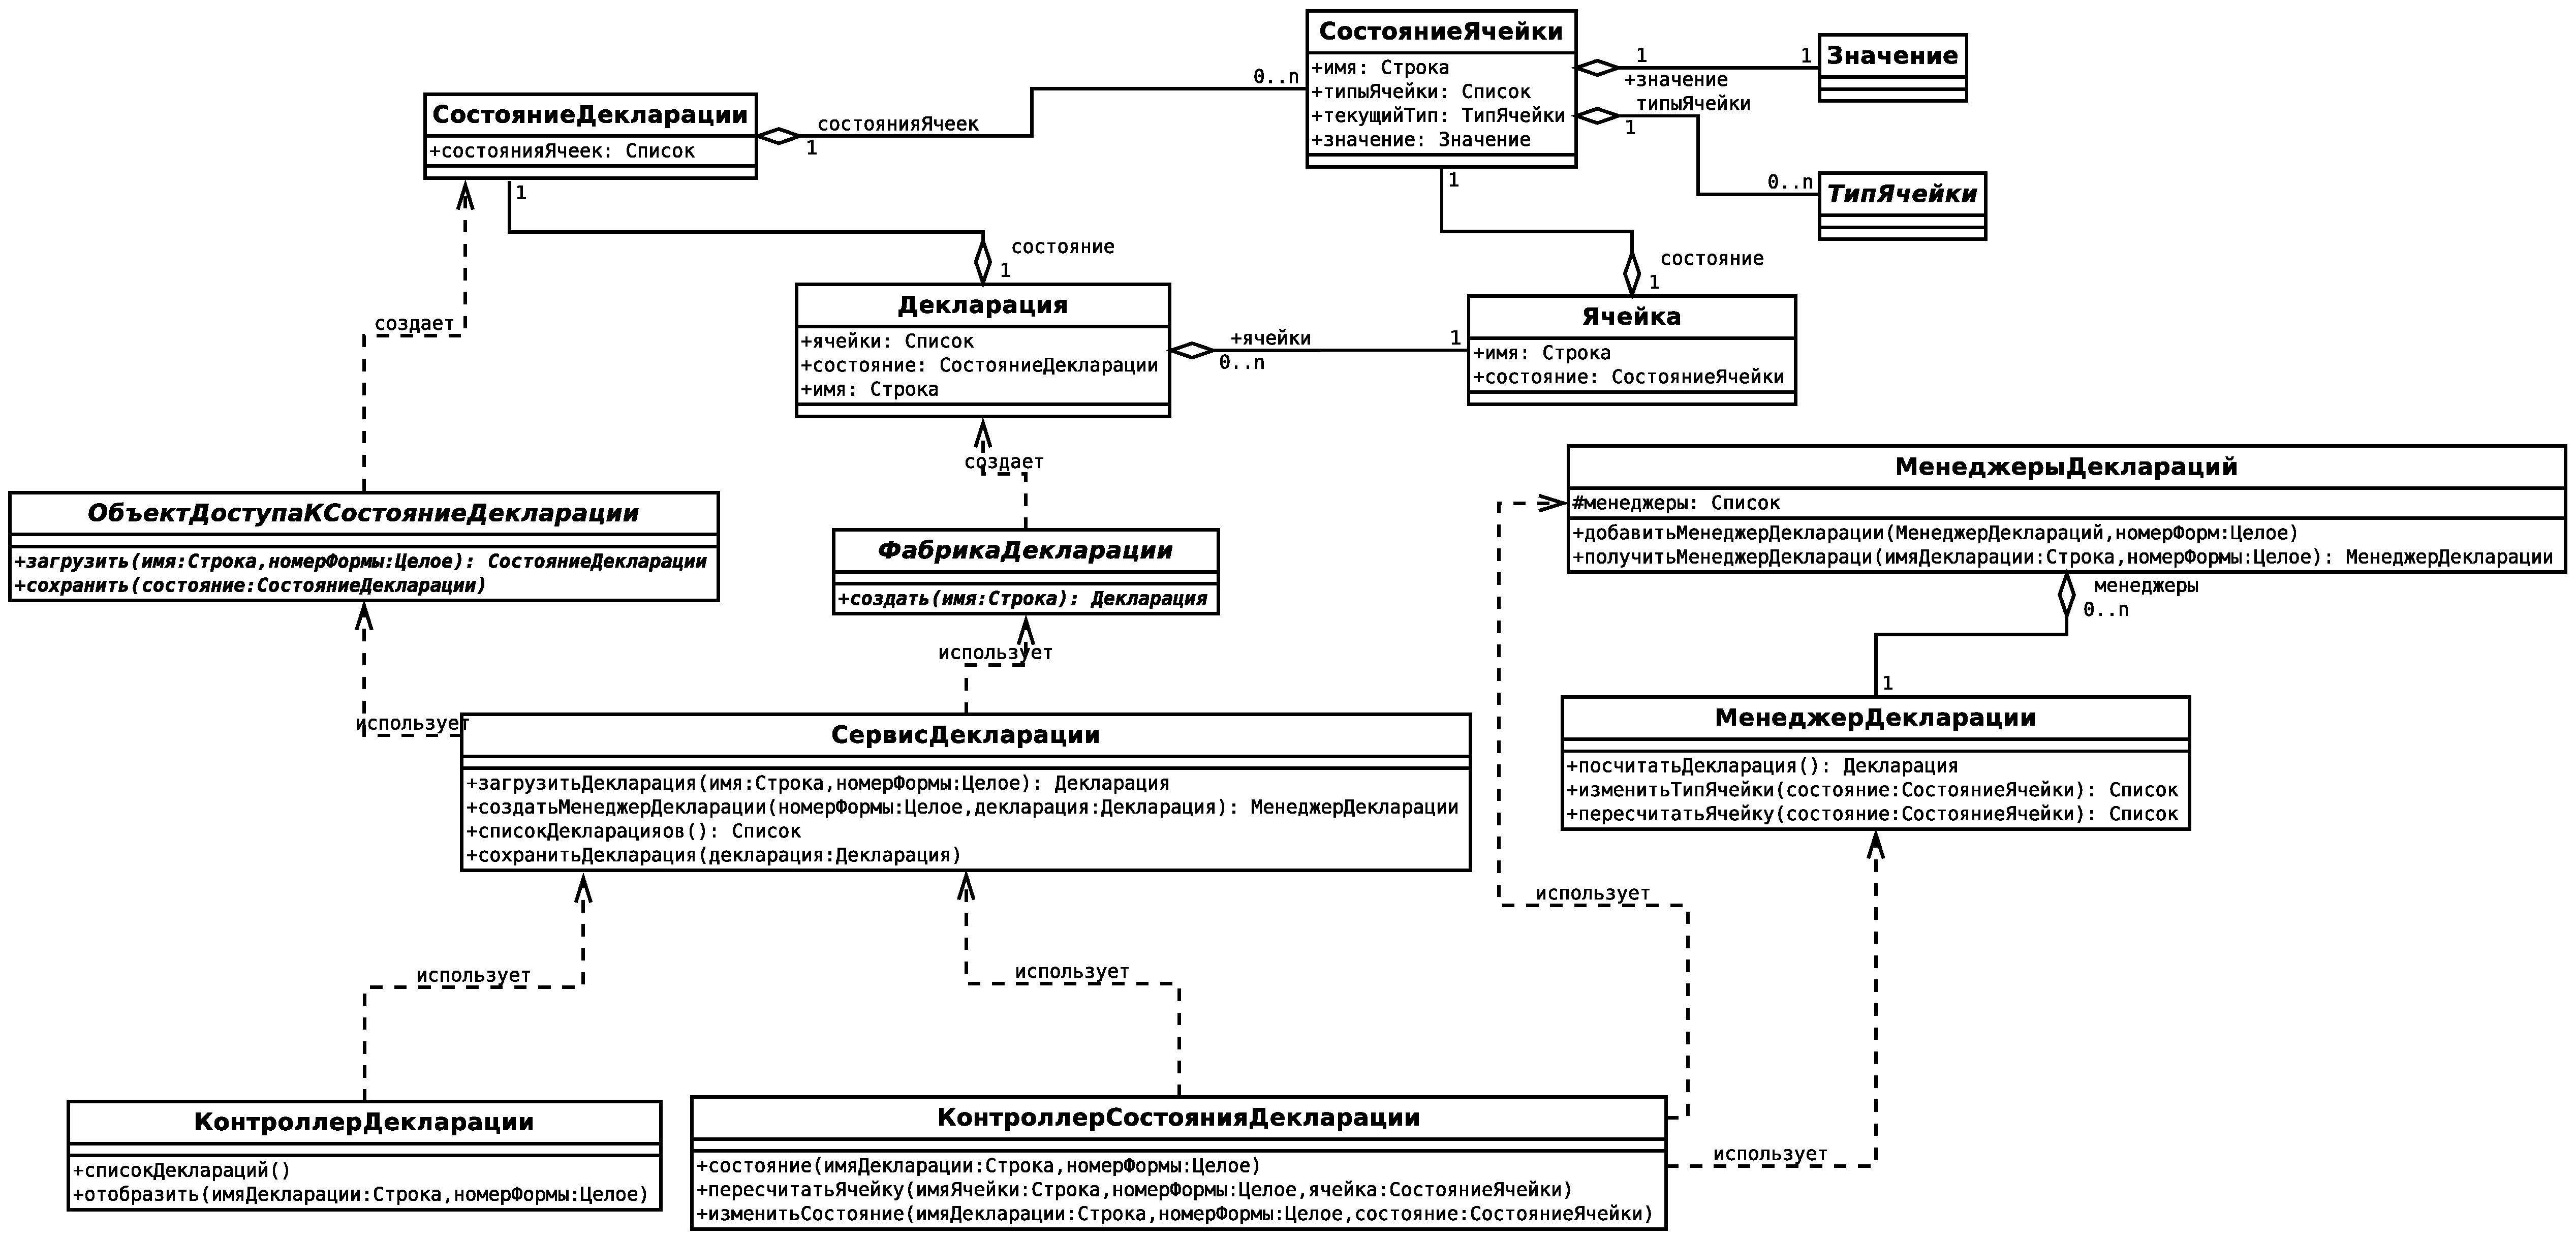
\includegraphics[scale=0.3]{uml/classes_1}
  \caption{Диаграмма классов}
  \label{pic:classes_1}
\end{sidewaysfigure}


На рисунке~\ref{pic:classes_2} представлена диаграмма, на которой изображена связь классов, которые используются ``Менеджером декларации''. ``Интерпретатор декларации'' используются для подсчета значений на ``Декларации'' для подсчета значений каждой ячейки используется ``Интерпретатор Ячейки'' - абстрактный класс, который содержит абстрактный метод ``посчитать'', параметрами являются экземпляры классов ``Тип Ячейки'' и ``Контекст'', как было описано во время анализа диаграммы сущность-связь, данный класс содержит информацию о правилах подсчета ячейки. Класс ``Интерпретаторы Ячеек'' содержит метод посчитать, который использует конкретную реализацию класса ``Интерпретатор Ячейки'' для подсчета значения, конкретная реализация выбирается в зависимости от ``ТипаЯчейки''.Абстрактный класс ``Контекст'' используется для хранения значений в рамках одного интерпретатора, например, для подсчета формулы необходимо получить значения ячеек, от которых зависит формула, класс был сделан по причине того, что значения могут получаться из состояний других деклараций, то есть можно сделать несколько реализаций данного класса для разных стратегий получения значений.
\begin{figure}
  \centering
  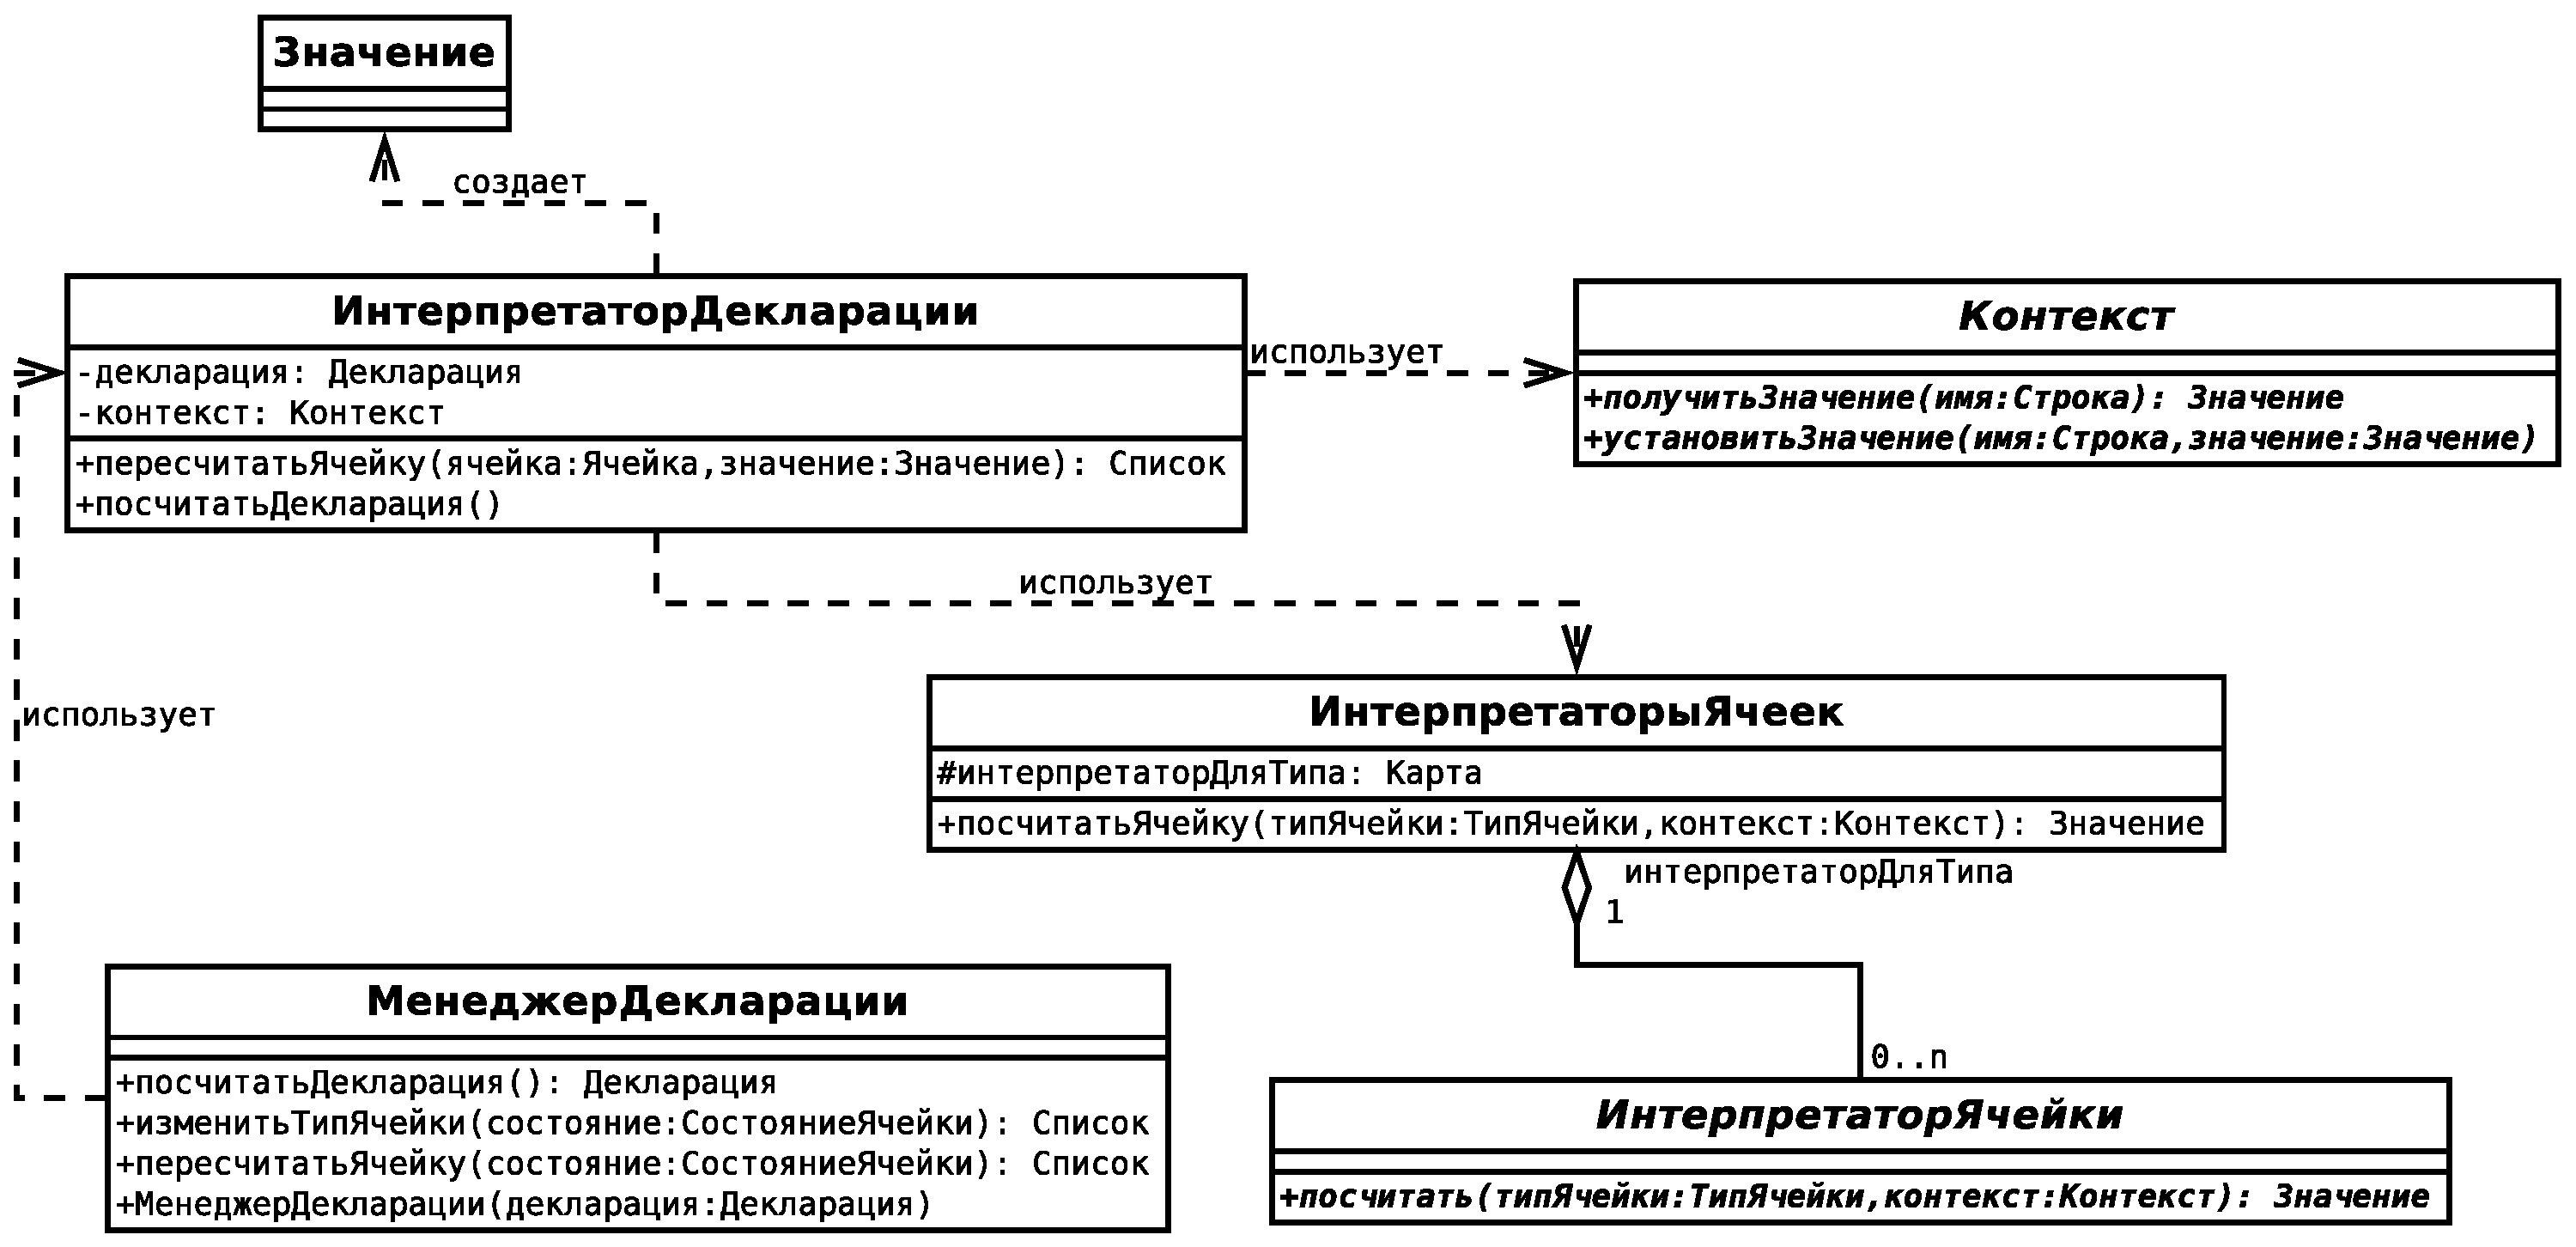
\includegraphics[scale=0.3]{uml/classes_2}
  \caption{Диаграмма классов}
  \label{pic:classes_2}
\end{figure}


На рисунке~\ref{pic:classes_3} представлена диаграмма, на которой изображены реализации классов для подсчта ячеек различных типов. Классы ``ИнтерпретаторФормульнойЯчейки'' и ``ИнтерпретаторРедактируемойЯчейки'' реализовывают метод ``посчитать'' для ``ТипЯчейкиФормула'' и ``ТипЯчейкиРедактируемая'' соответственно. ``ИнтепретаторЯчейкиФормула'' использует класс ``ОценщикВыражения'' который предоставляет статические методы ``получитьПеременные'' и ``оценить''. Метод ``получитьПеременные'' возвращает все переменные выражения, которые потребуются для подсчета выражения. Метод ``оценить'' возвращает значение выражение, параметр ``контекст'' является картой, в которой ключом являются названия переменных, а значением - объект, который показывает значение переменных. ``ОценщикВыражения'' использует класс ``СинтаксическийАналализаторВыражения'', который используется для анализа выражений, метод ``анализировать'' возвращает абстрактное синтаксическое дерево, которое затем обрабатывается для вычисления значения выражения. ``СинтаксическийАнализаторВыражения'' использует класс ``ЛексическийАнализаторВыражения'' для получения лексем, метод ``получитьЛексему'' получает следующую лексему из потока данных (в данном случае - строка), которая используется синтаксическим анализатором, для анализа выражения.
\begin{figure}
  \centering
  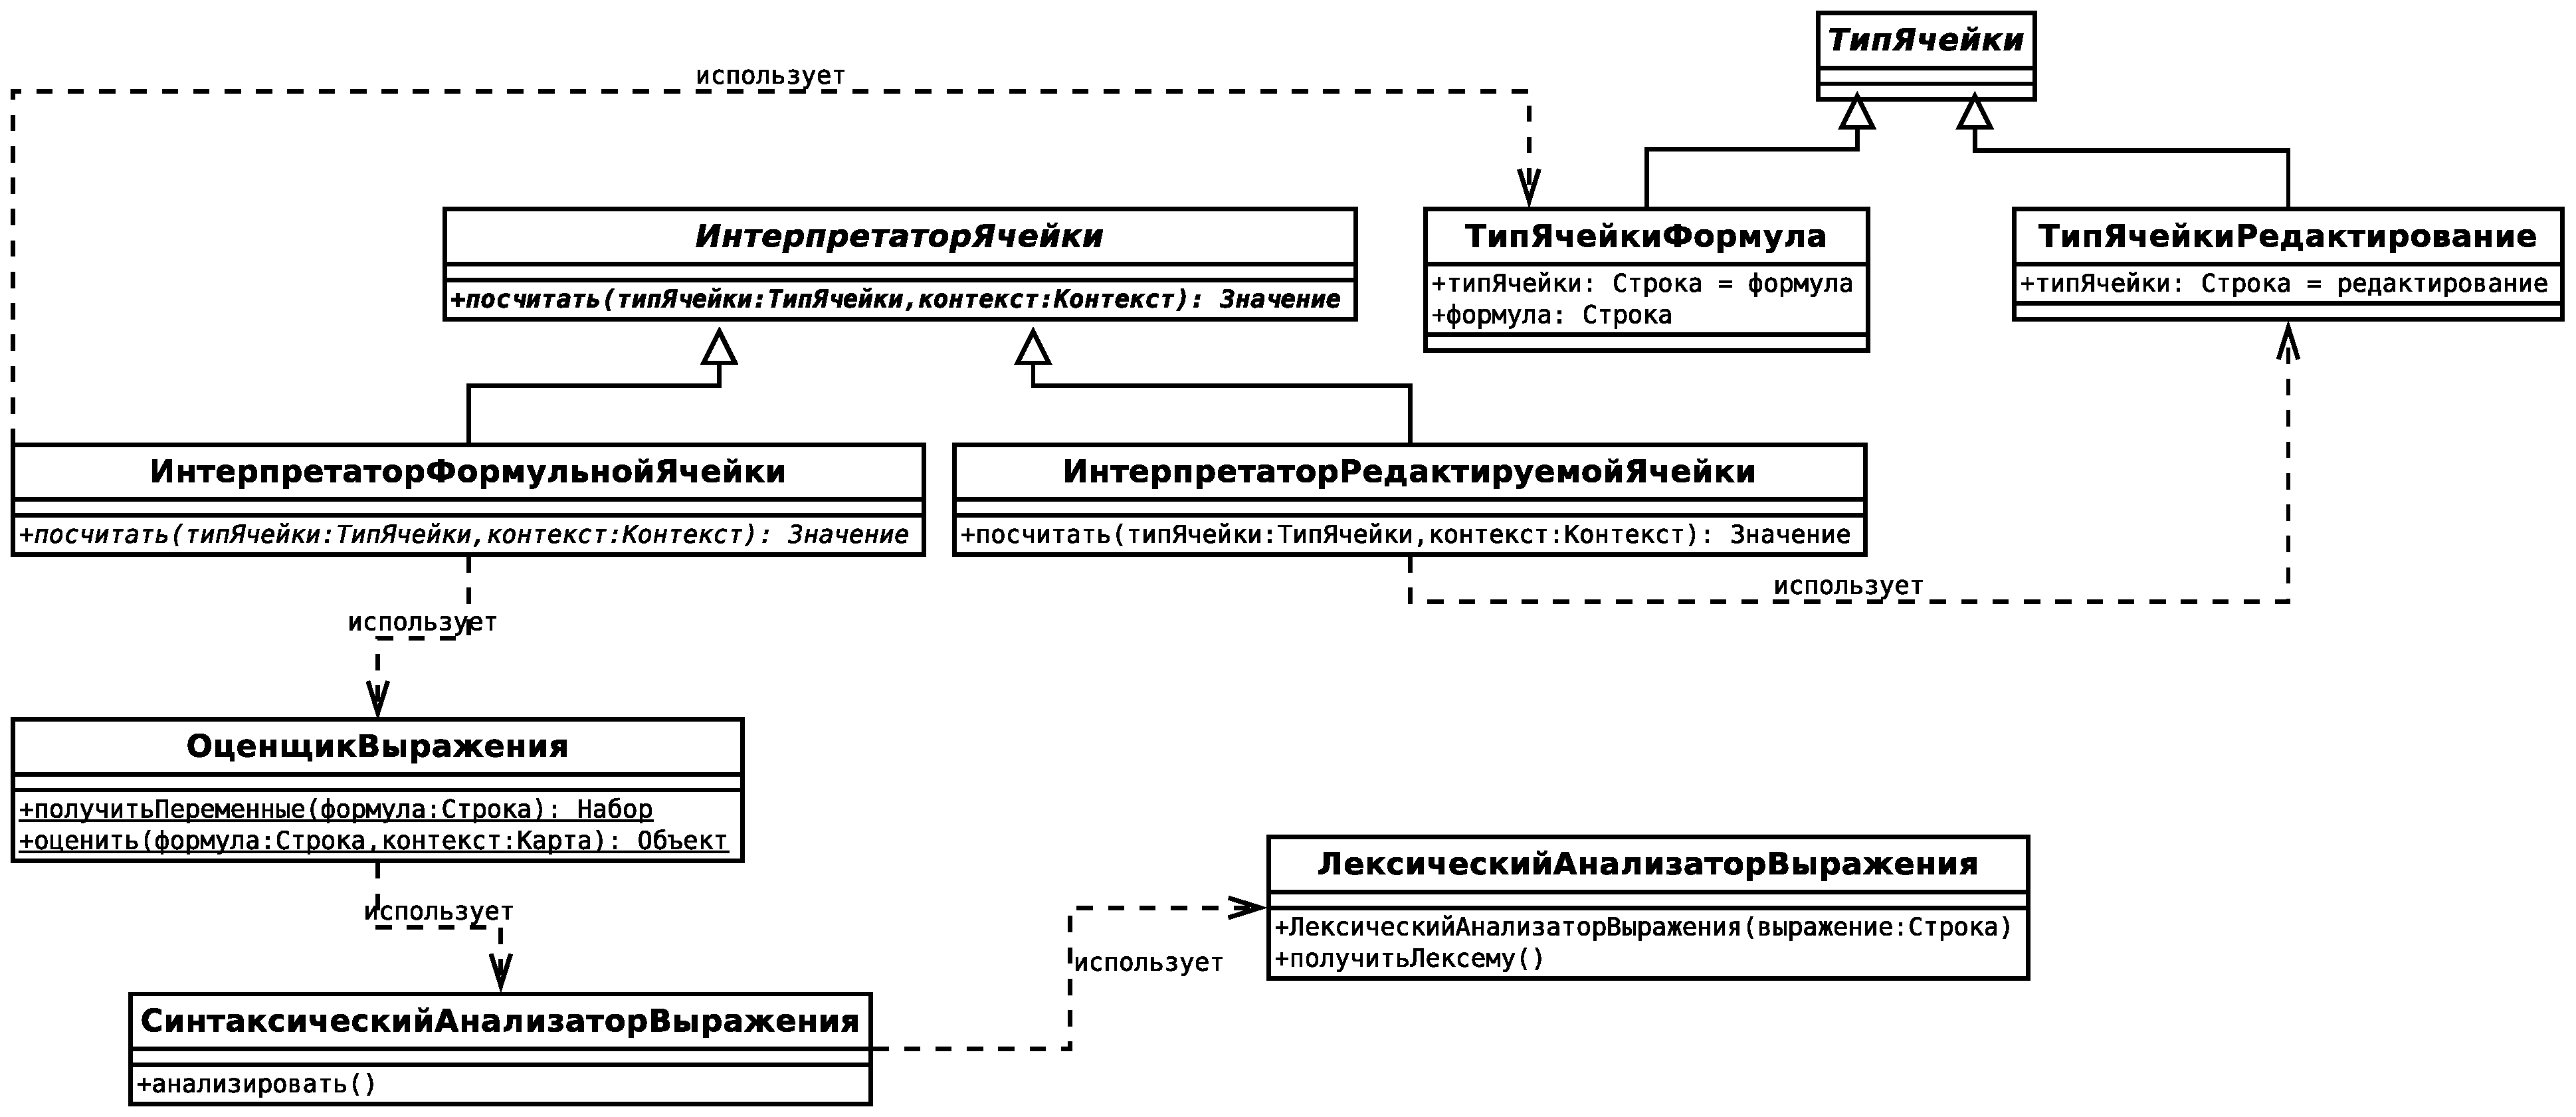
\includegraphics[scale=0.26]{uml/classes_3}
  \caption{Диаграмма классов}
  \label{pic:classes_3}
\end{figure}


На рисунке~\ref{pic:classes_4} представлена диаграмма классов, которые используются для отображения декларации. Введем стереотип ``ПИ'' (``Пользовательский Интерфейс'') который представляет пользовательский интерфейс приложения, в данном случае - это динамическая сгенерированная веб-страница. ``СтраницаДекларации'' должна содержать представление декларации, для представления декларации она использует класс ``РаспознавательВидаДекларации'' который предоставляет ``ВидДекларации'' для конкретного объекта, ``ВидДекларации'' сожержит метод ``получитьВид'', который принимает параметр ``писатель'' типа ``Писатель'', данный тип предоставляет интерфейс для вывода в выходной поток(язык программирования Java в стандартной библиотеке имеет класс ``Writer''). Метод ``получитьВид'' выводит в поток отображение декларации в каком-либо формате. ``РаспознавательВидаДекларации'' и ``ВидДекларации'' содержать абстрактные методы, которые должны быть реализованы для конкретного вида отображения декларации. ``РаспознавательВидаДекларации'' содержит метод ``распознать'' который возвращает конкретную реализацию класса ``ВидДекларации''. Метод распознать в качестве параметра принимает экземпляр класса ``Декларация'', который требуется отобразить.
\begin{figure}
  \centering
  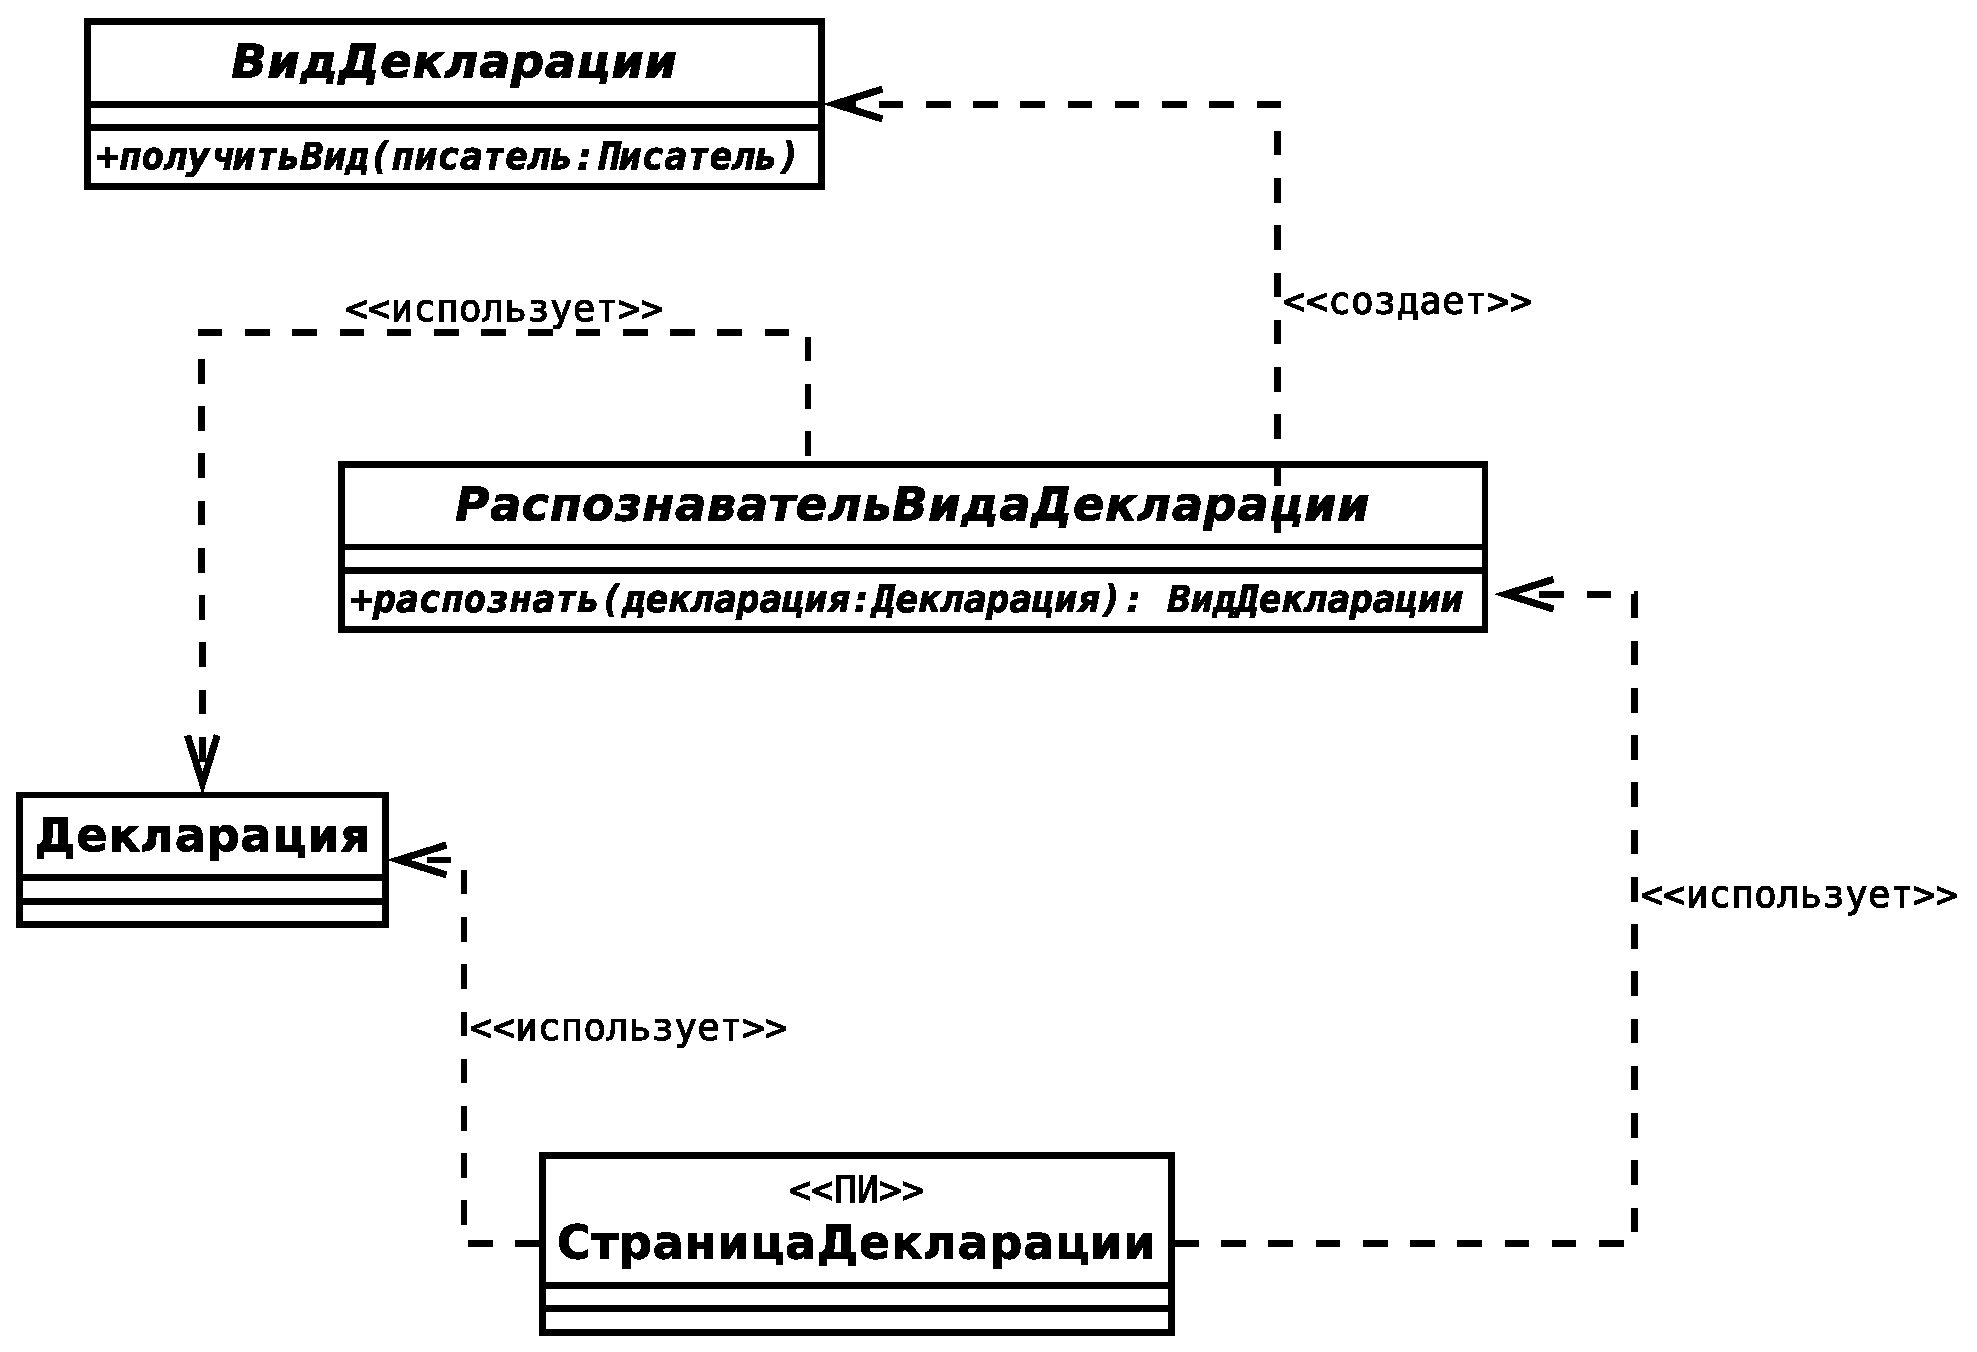
\includegraphics[scale=0.5]{uml/classes_4}
  \caption{Диаграмма классов}
  \label{pic:classes_4}
\end{figure}
\section{Детализация вариантов использования}
Проведем детализацию вариантов использования, для того чтобы отобразить выделенные варианты во взаимодействие между представленными классами системы.


Введем стереотип ``ПИ''(``Пользовательский Интерфейс'') для представления интерфейса пользователя, через который пользователь будет взаимодействовать с системой. К системе было предъявлено требование о предоставлении веб-интерфейса. Проектируемая система будет представлять собой клиент-серверное приложение, где клиентом будет являться браузер, а вся вычислительная логика будет реализована на сервере.


После того, как клиент отправит HTTP запрос, управление будет передано соответствующему контроллеру. В качестве ответа контроллер может вернуть идентификатор веб-страницы, которую требуется отобразить и передать какие-то данные клиенту. В данном случае стереотип ``ПИ'' будет представлять собой веб-страницу. Стереотип ``контроллер'' будет представлять собой класс, который обрабатывает запросы клиента.Сообщения от ``ПИ'' контроллеру и от контроллера передаются(принимаются) в асинхронном режиме. Для реализации асинхронных запросов требуется использовать технологию AJAX (Asynchronous JavaScript and XML), в настоящий момент существует несколько библиотек, которые позволяют использовать эту технолгию.


На рисунке~\ref{pic:sequence_1} представлена диаграмма последовательности для варианта использования ``Создание декларации''. Когда пользователь запрашивает список деклараций, у контроллера вызывается метод ``списокДеклараций'', ``КонтроллерДекларации'' вызывает метод ``списокДеклараций'' класса ``СервисДекларации'', затем контроллер передает управление странице ``СписокДеклараций''. Пользователь выбирает декларацию, который он хочет загрузить, ``СписокДеклараций'' передает управление методу ``отобразить'' контроллера. Контроллер вызывает метод ``загрузитьДекларация'' ``СервисаДекларации'', который возвращает экземпляр класса ``Декларация'', который передается странице ``Декларация''. ``Декларация'' запрашивает состояние декларации, вызвав метод ``состояние'' контроллера ``КонтроллерСостоянияДекларации''. Контроллер вызывает метод ``загрузитьДекларация'' у ``СервисДекларации'', который возвращает декларацию, далее контроллер вызывает метод ``создатьМенеджерДекларации'' класса, ``СервисДекларации'', который создает ``МенеджерДекларации'', далее контроллер вызывает метод ``посчитатьДекларация'' класса ``МенеджерДекларации'', который считает ``Декларация'' , и устанавливает соответствующее ``СостояниеДекларации''. Далее контроллер взывает метод ``добавитьМенеджерДекларации'' для того что бы сохранить ``МенеджерДекларации'' в оперативной памяти для того, что бы использовать его для дальнейших операций с ``СостояниемДекларации''. Управление передается странице ``Декларация''.

\begin{sidewaysfigure}
  \centering
  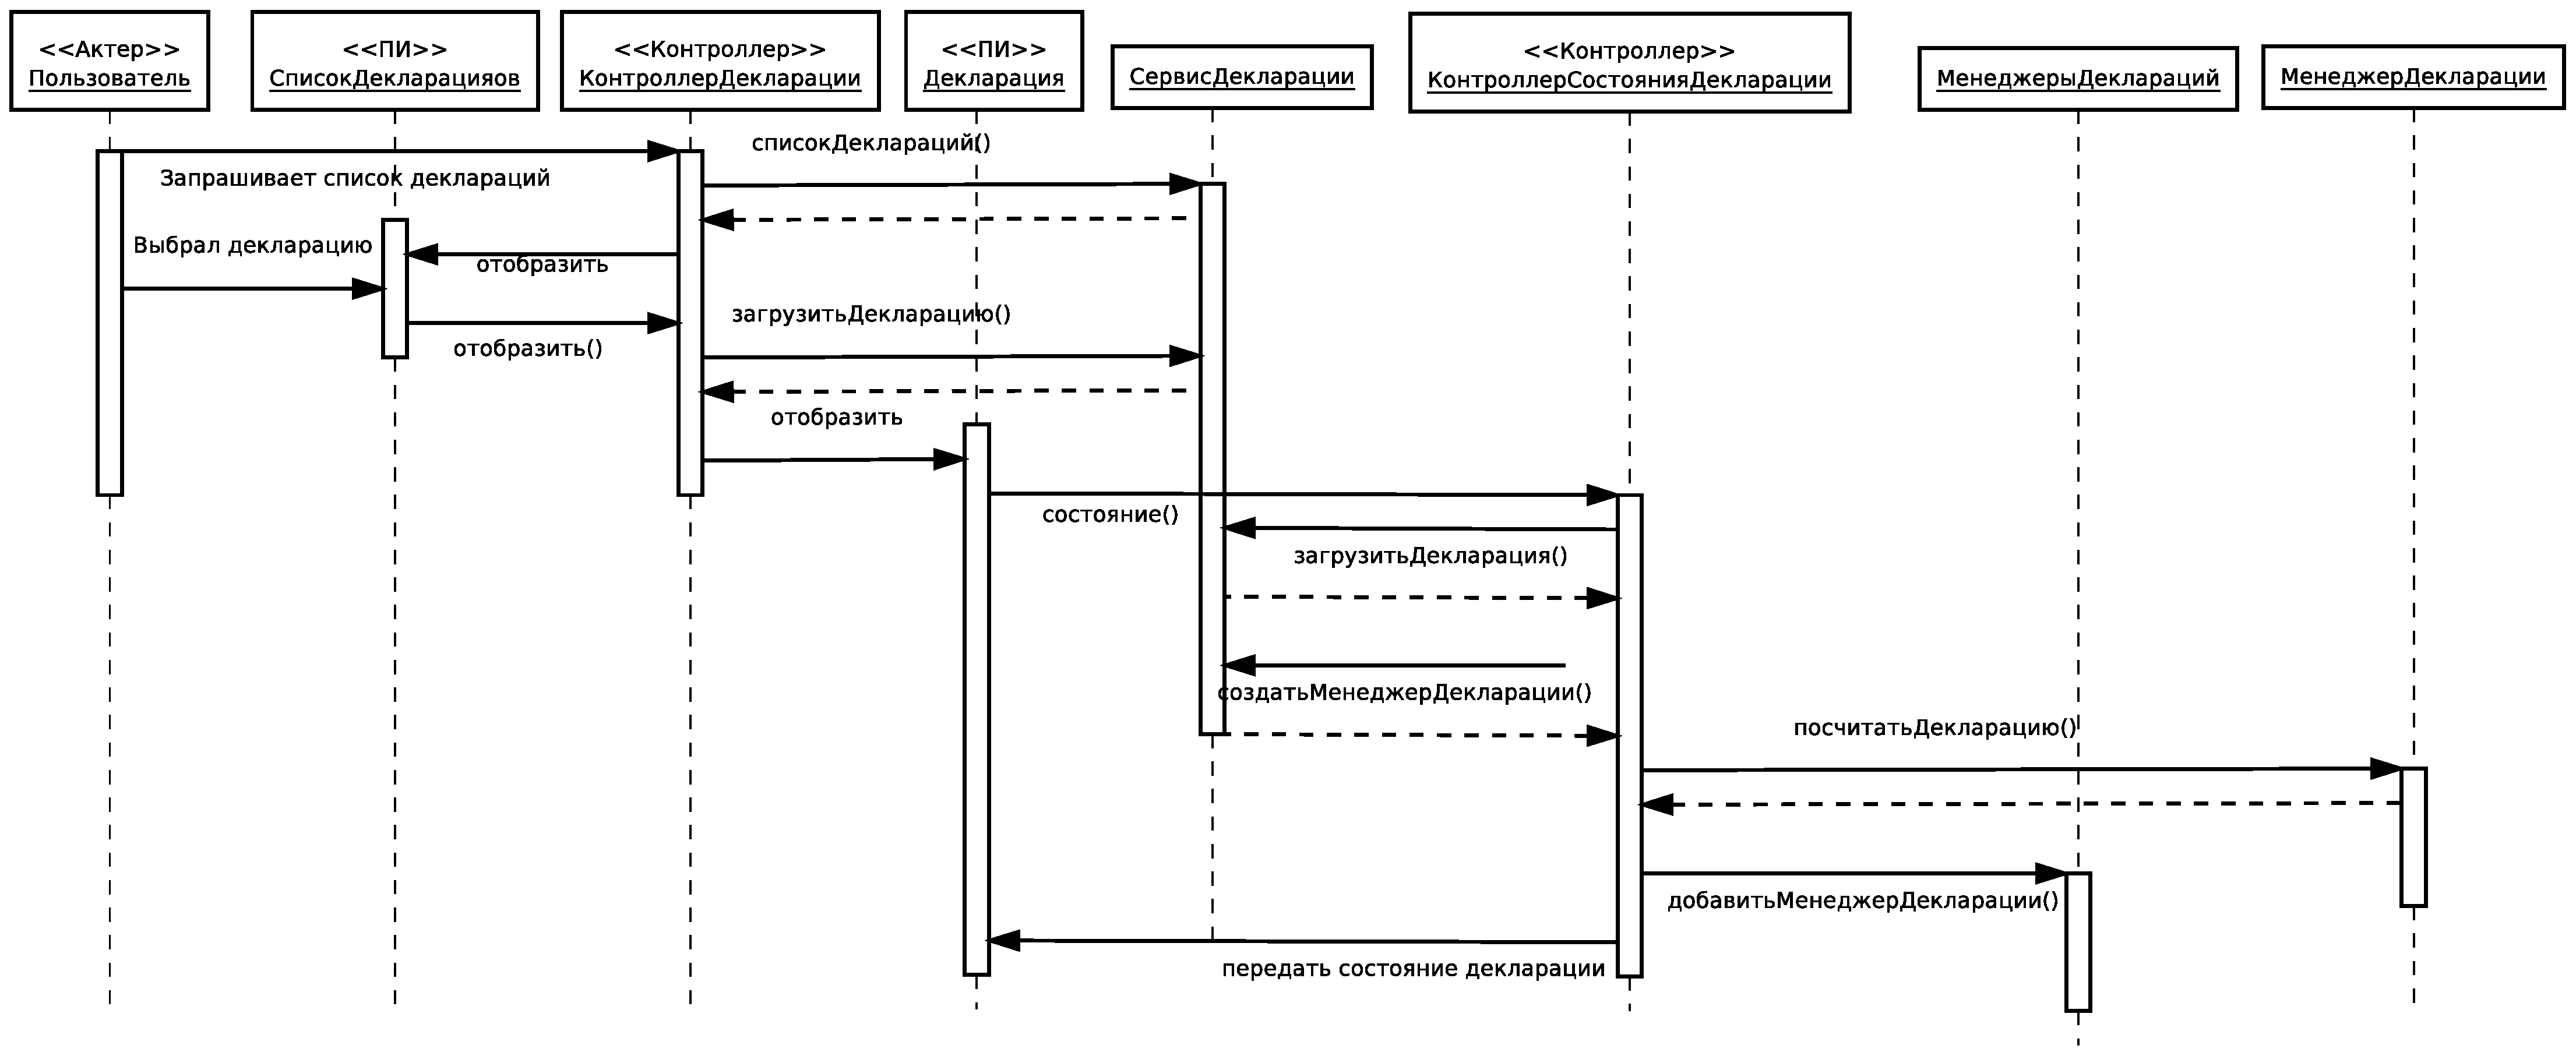
\includegraphics[scale=0.35]{uml/sequence_1}
  \caption{Диаграмма последовательности для создания декларации}
  \label{pic:sequnce_1}
\end{sidewaysfigure}
На рисунке~\ref{pic:sequence_2} представлена диаграмма последовательности для варианта использования ``Пересчитать значение''. Пользователь находится на странице ``Декларация'' для пересчета значения ячейки пользователь вводит новое значение, страница посылает запрос контроллеру, который содержит новое состояние ячейки (в ``СостояниеЯчейки'' изменилось ``Значение'') контроллер ``КонтроллерСостоянияДекларации'' получает ``МенеджерДекларации'', который был создан при получении значений для декларации. Контроллер вызывает метод ``пересчитатьЯчейку'' у ``МенеджерДекларации'', в качестве параметра для метода передается ``СостояниеЯчейки'' которое было получено. Метод возвращает список пересчитанных ячеек (список содержит экземпляры класса ``Ячейка''). Контроллер возвращает этот список странице ``Декларация'' в качестве ответа на асинхронный запрос.

\begin{sidewaysfigure}
  \centering
  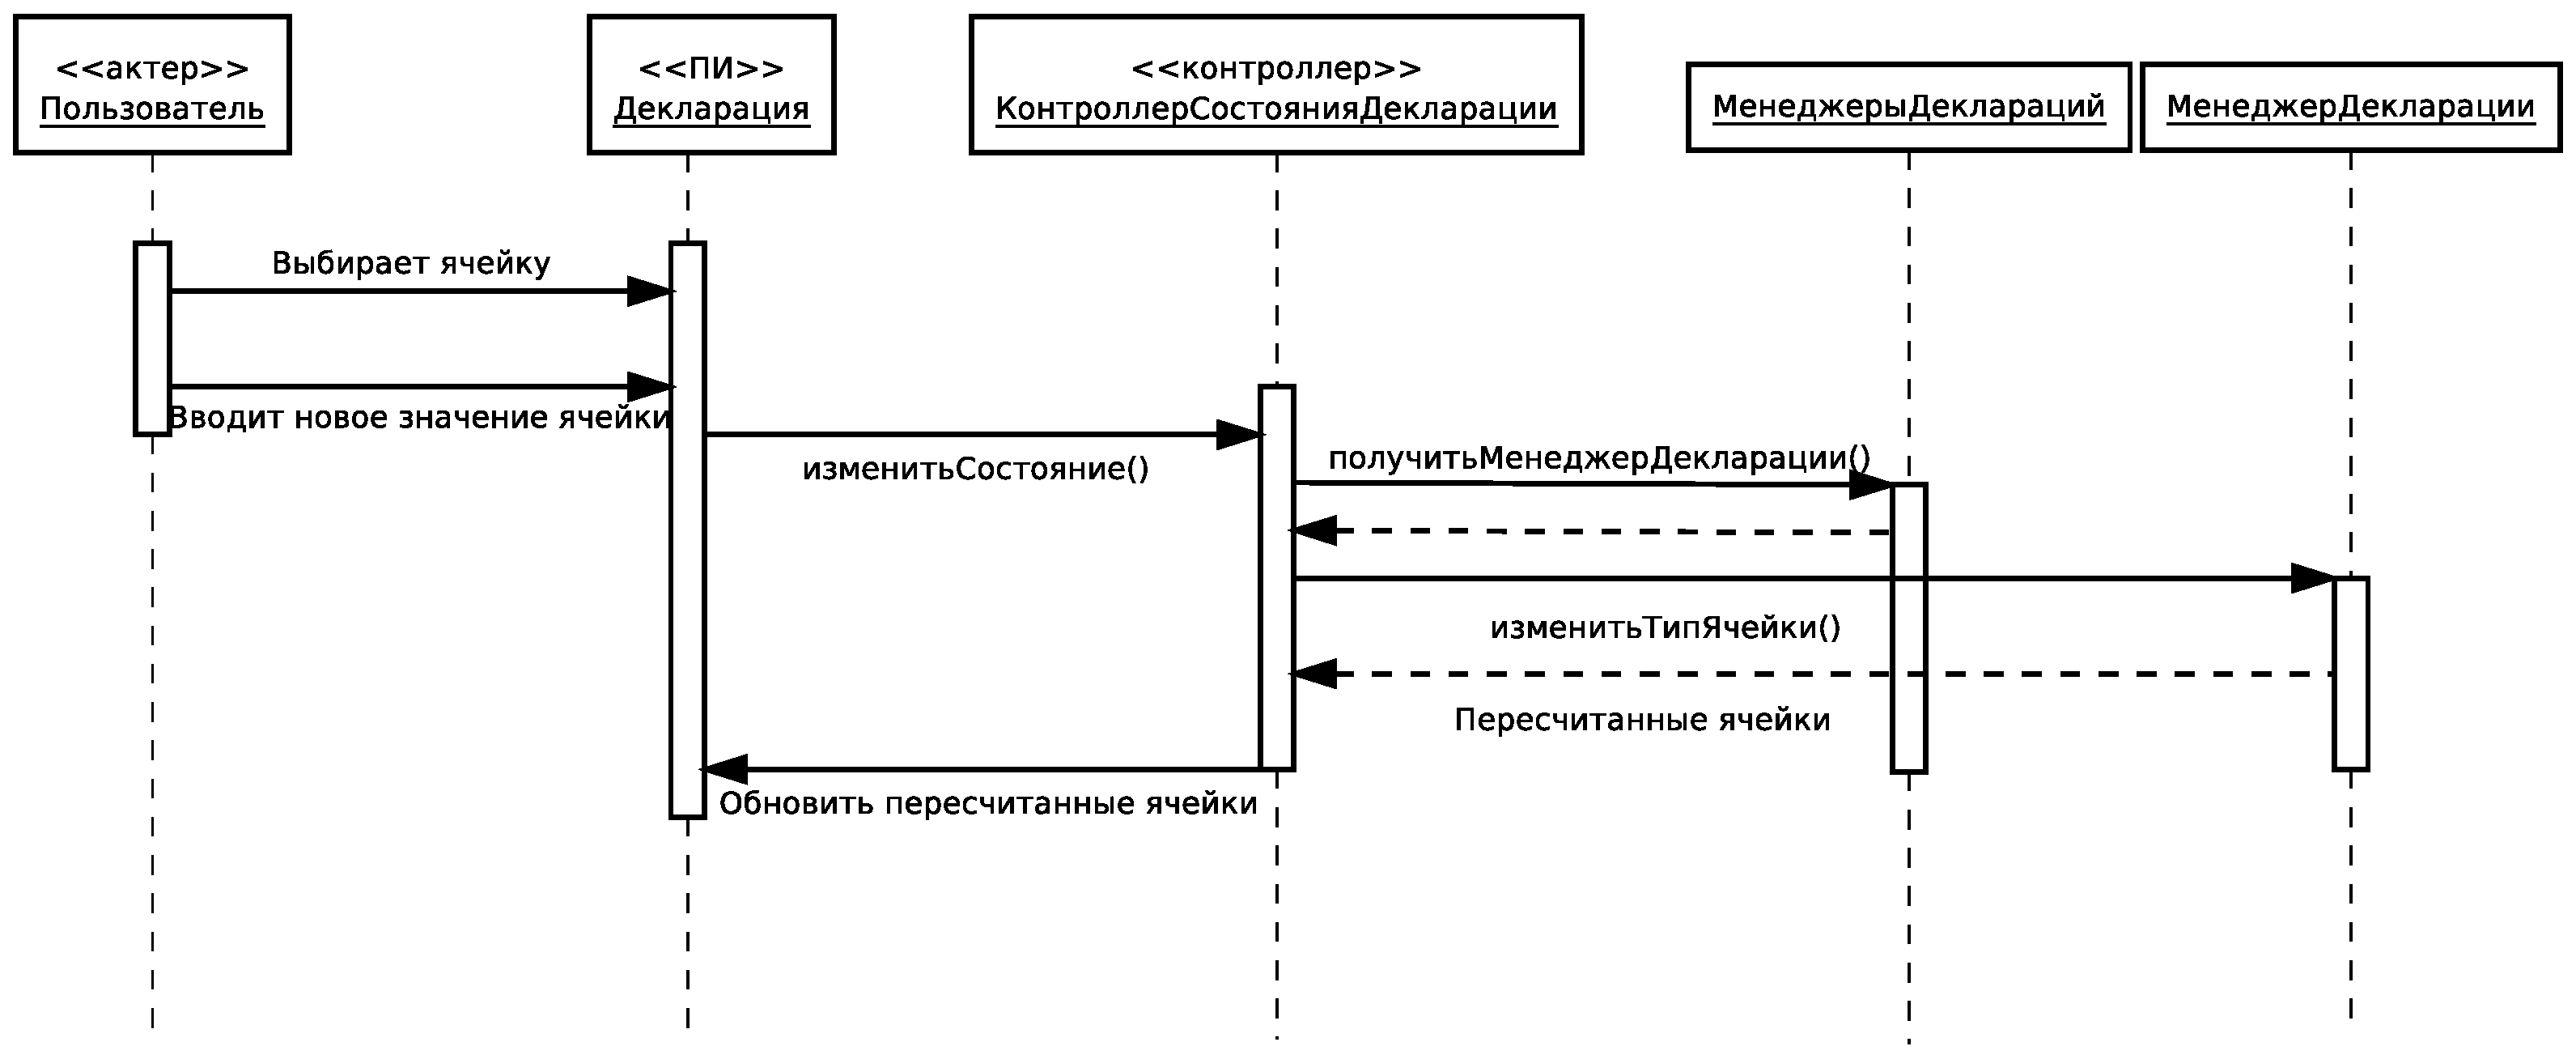
\includegraphics[scale=0.4]{uml/sequence_2}
  \caption{Диаграмма последовательности для пересчета ячейки}
  \label{pic:sequence_2}
\end{sidewaysfigure}

На рисунке~\ref{pic:sequence_3} представлена диаграмма последовательности для варианта использования ``Изменить тип ячейки''. Пользователь находится на странице ``Декларация''. При изменении состояния ячейки страница посылает асинхронный запрос, который обрабатывает метод ``изменитьСостояние'' контроллера ``КонтроллерСостоянияДекларации''. Контроллер получает экземпляр класса текущего ``МенеджераДекларации'', у которого вызывает метод ``изменитьТипЯчейки''. Метод возвращает список из пересчитанных ячеек. Контроллер возвращает полученный список в качестве ответа на асинхронный запрос страницы ``Декларация''.

\begin{sidewaysfigure}
  \centering
  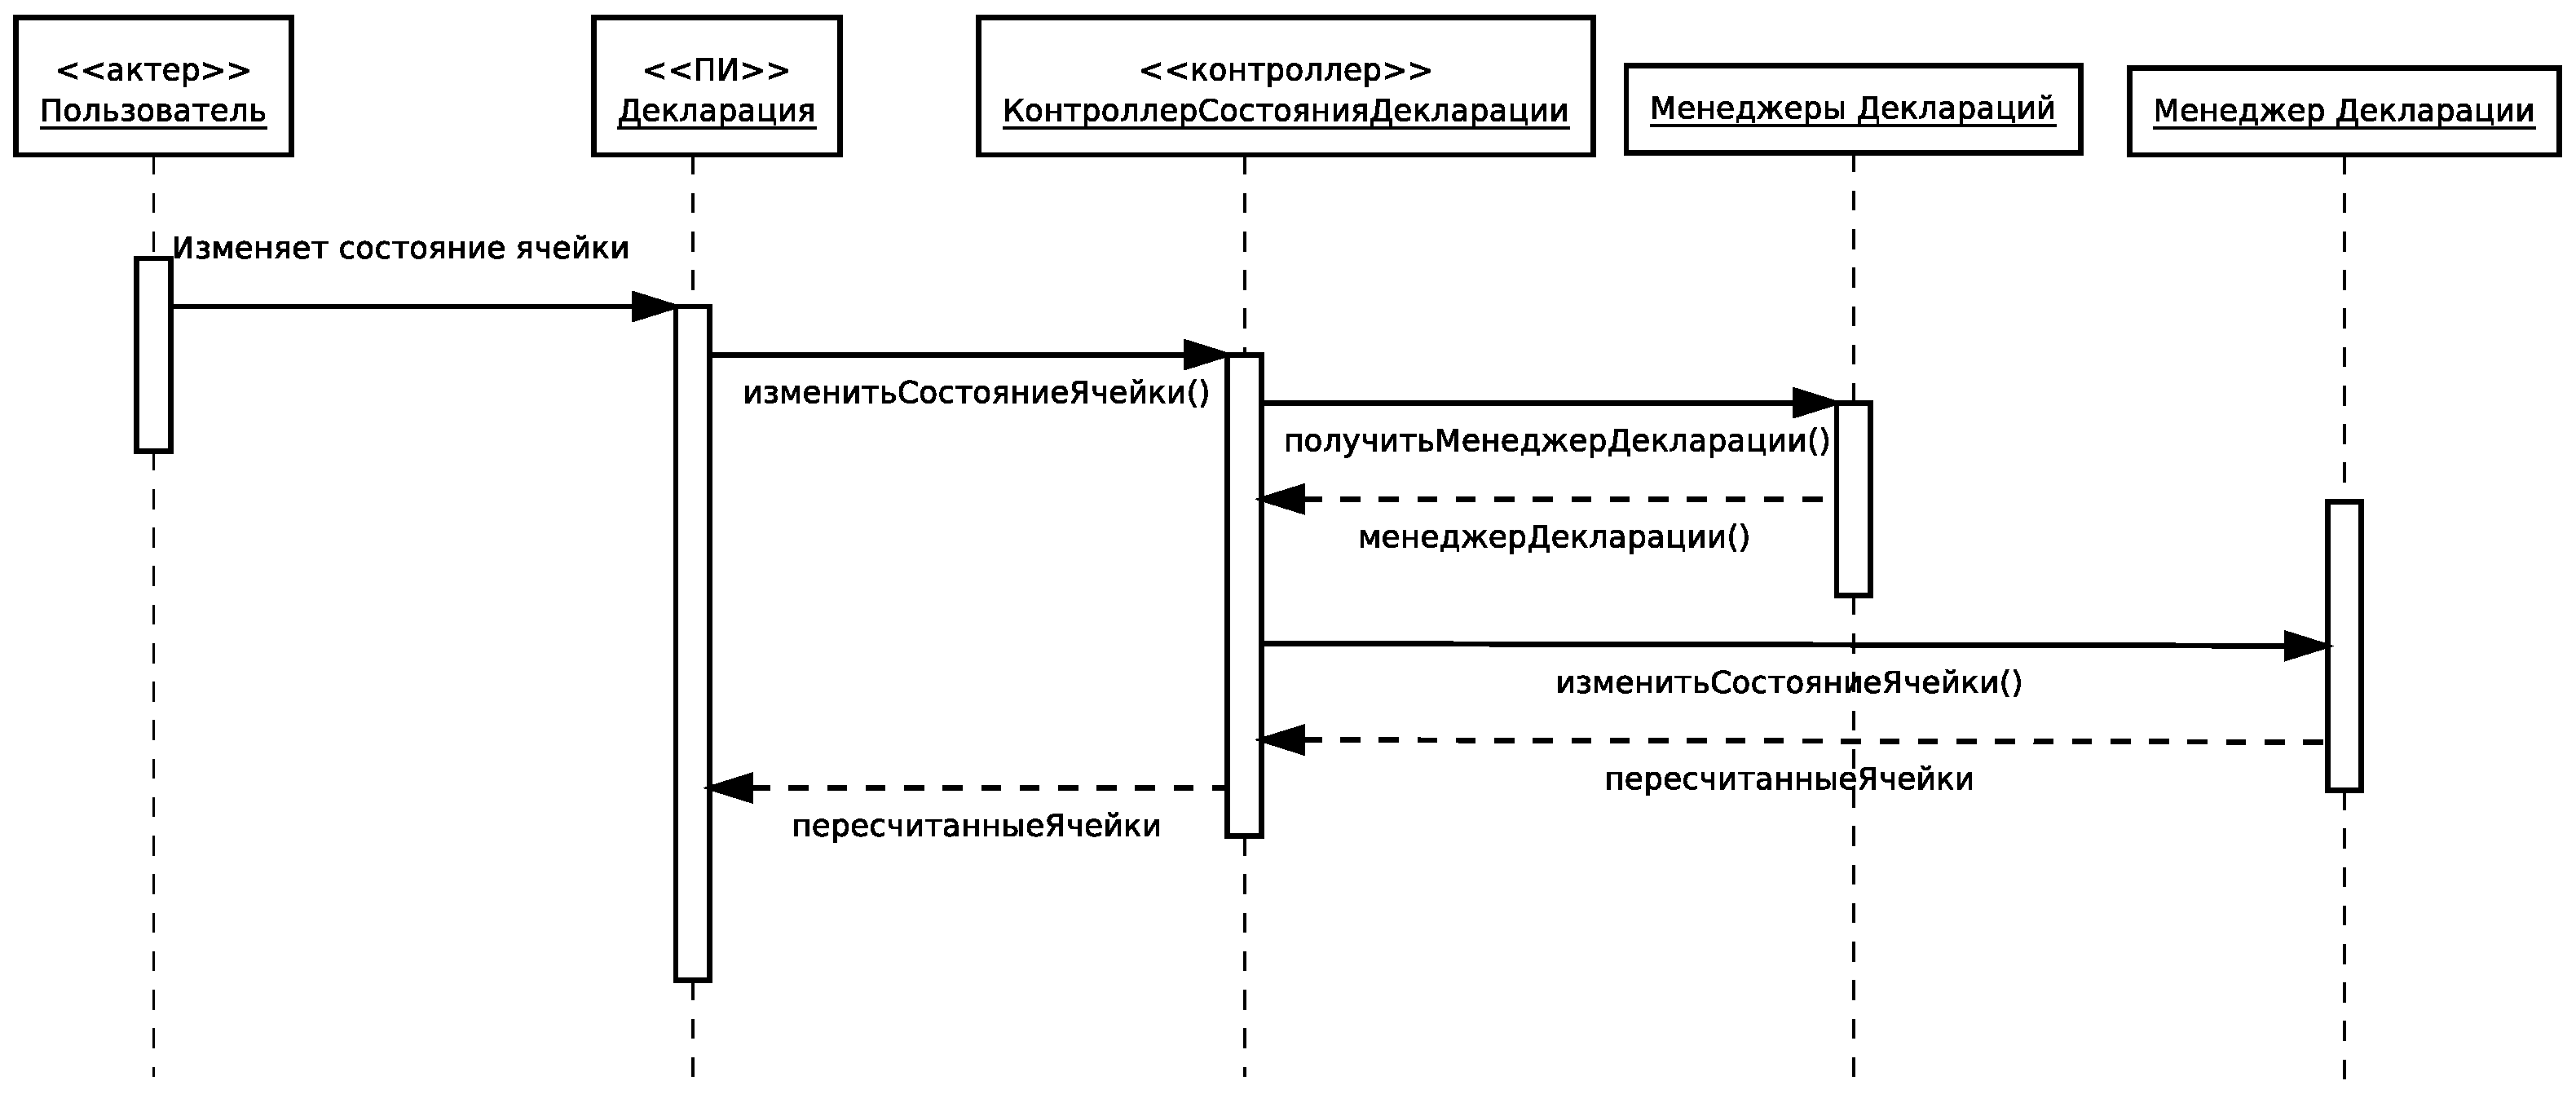
\includegraphics[scale=0.4]{uml/sequence_3}
  \caption{Диаграмма последовательности для изменения типа ячейки}
  \label{pic:sequence_3}
\end{sidewaysfigure}

\textbf{Аннотация: далее следует диаграмма состояния для системы}

\section{Представление декларации в формате XML}
Для физического представления декларации был выбран язык XML. XML — это иерархическая структура, предназначенная для хранения любых данных. Визуально структура может быть представлена как дерево. Важнейшее обязательное синтаксическое требование заключается в том, что документ имеет только один корневой элемент. Это означает, что текст или другие данные всего документа должны быть расположены между единственным начальным корневым тегом и соответствующим ему конечным тегом.


Для описания семантики декларации необходимо описать свойства объектов: ``Декларация'', ``Ячейка'', свойство ``ТипыЯчеек'' (что является списком, который содержит объекты типа ``ТипЯчейки'') объекта ``СостояниеЯчейки''. Свойства ``Декларации'' возможно выделить в иерархическую структуру (рисунок~\ref{pic:report_hierarchy}).
\begin{figure}
\begin{verbatim}
\Декларация
    \Имя
    \Ячейки
       \Ячейка
          \Имя ячейки
          \Тип данных
          \Состояние ячейки
              \Типы ячейки
                 \Тип ячейки
\end{verbatim}
\caption{Представление свойств объекта ``Декларация'', которые требуется сохранить в формате XML, в виде иерархической структуры}
\label{pic:report_hierarchy}
\end{figure}
Представим данную структуру в формате XML:
\begin{figure}
  \begin{verbatim}
    <?xml version="1.0"?>
    <report>
       <name>Название декларации</name>
       <cells>
          <cell>
            <name>имя ячейки</name>
            <cellState>
               <types>
                 <type.название_типа_ячейки>
                    <!-- свойства типа -->
                 </type>
                 <!-- .... -->
               </types>
            </cellState>
          </cell>
          <!-- .... -->
       </cells>
    </report>
  \end{verbatim}
  \caption{Представление объекта ``Декларация'' в формате XML}
\end{figure}

\section{Вывод}

\textbf{Аннотация: будет подведен итог проектирования системы с указанием проделанной работы}

\chapter{Реализация системы создания и управления электронными налоговыми декларациями}

\section{Выбор и обоснование средств разработки}
Для реализации системы документооборота использовался язык программирования Java. Java - объектно-ориентированный язык программирования, разрабатываемый компанией Sun Microsystems.Программы на Java транслируются в байт-код, выполняемый виртуальной машиной Java (JVM) — программой, обрабатывающей байтовый код и передающей инструкции оборудованию как интерпретатор, но с тем отличием, что байтовый код, в отличие от текста, обрабатывается значительно быстрее.
Достоинство подобного способа выполнения программ — в полной независимости байт-кода от операционной системы и оборудования, что позволяет выполнять Java-приложения на любом устройстве, для которого существует соответствующая виртуальная машина. Другой важной особенностью технологии Java является гибкая система безопасности благодаря тому, что исполнение программы полностью контролируется виртуальной машиной. Любые операции, которые превышают установленные полномочия программы (например, попытка несанкционированного доступа к данным или соединения с другим компьютером) вызывают немедленное прерывание.
Особенности языка:
\begin{itemize}
  \item автоматическое управление памятью
  \item расширенные возможности обработки исключительных ситуаций
  \item богатый набор средств фильтрации ввода/вывода
  \item набор стандартных коллекций, таких как массив, список, стек и т.д.
  \item наличие простых средств создания сетевых приложений (в том числе с использованием протокола RMI)
  \item наличие классов, позволяющих выполнять HTTP-запросы и обрабатывать ответы
  \item встроенные в язык средства создания много-поточных приложений
\end{itemize}
Следует отметить, что для данного языка существует большое количество библиотек, распространяемых под свободными лицензиями, для работы с различными форматами файлов, работы с базами данных, для разработки пользовательских интерфейсов, написания приложений, использующих веб-интерфейс и т.д.

\section{Выбор инструментальных средств разработки}

\subsection{Spring}
Spring - open source фреймворк для Java-платформы. Первая версия была написана Родом Джонсоном, который впервые опубликовал её вместе с изданием своей книги ``Expert One-on-One Java EE Design and Development''
Фреймворк был впервые выпущен под лицензией Apache 2.0 license в июне 2003 года. Первый стабильный релиз 1.0 был выпущен в марте 2004. Последующие стабильные релизы вышли в сентябре 2004 года и марте 2005 года.
Несмотря на то, что Spring Framework не обеспечивал какую-либо конкретную модель программирования, он стал широко распространённым в Java сообществе главным образом как альтернатива и замена модели Enterprise JavaBeans. Spring Framework предоставляет большую свободу Java разработчикам в проектировании, кроме того, он предоставляет хорошо документированные и лёгкие в использовании решения проблем, возникающих при создании приложений промышленного масштаба.
Между тем, особенности ядра Spring Framework применимы в любом Java приложении, и существует множество расширений и усовершенствований для построения веб-приложений на Java Enterprise платформе. По этим причинам Spring приобрёл большую популярность и признаётся разработчиками как стратегически важный фреймворк.
(Аннотация: диаграмма модулей Spring Framework и перечисление используемых модулей SF в системе)

\subsection{Hibernate}
Hibernate — библиотека для языка программирования Java, предназначенная для решения задач объектно-реляционного проецирования (object-relational mapping — ORM). Она представляет собой свободное программное обеспечение с открытым исходным кодом , распространяемое на условиях GNU Lesser General Public License. Данная библиотека предоставляет лёгкий в использовании каркас (фреймворк) для отображения объектно-ориентированной модели данных в традиционные реляционные базы данных.
Целью Hibernate является освобождение разработчика от значительного объёма сравнительно низкоуровневого программирования по обеспечению хранения объектов в реляционной базе данных. Разработчик может использовать Hibernate как в процессе проектирования системы классов и таблиц ``с нуля'', так и для работы с уже существующей базой данных.
Hibernate не только решает задачу связи классов Java с таблицами базы данных (и типов данных Java с типами данных SQL), но также предоставляет средства для автоматической генерации и обновления набора таблиц, построения запросов и обработки полученных данных и может значительно уменьшить время разработки, которое обычно тратится на ручное написание SQL- и JDBC-кода. Hibernate автоматизирует генерацию SQL-запросов и освобождает разработчика от ручной обработки результирующего набора данных и преобразования объектов, максимально облегчая перенос (портирование) приложения на любые базы данных SQL.
Hibernate обеспечивает прозрачную поддержку сохранности данных  для ``POJO'' (то есть для стандартных Java-объектов). единственное строгое требование для сохраняемого класса — наличие конструктора по умолчанию (без параметров).
Hibernate используется как в standalone Java-приложениях, так и в приложениях на платформе Java EE, использующих сервлеты или EJB.
(Аннотация: описание того, как используется Hibernate в системе)

\section{Программная реализация компонентов системы}
Аннотация: приведена диаграмма развертывания системы, на которой изображены следующие узлы:
\begin{itemize}
  \item Сервер Приложений (сожержит компоненты autotaxes.war и autotaxes-engine.jar)
  \item Сервер Базы Данных (содержит компонент База Данных )
  \item Пользовательская Станция (содержит компонент Веб-браузер)
\end{itemize}
\subsection{Реализация классов системы}
Аннотация: представлены диаграммы на которых изображены реализации абстрактных классов системы и их описание:
\begin{itemize}
  \itemРеализация класса ``ЗагрузчикДекларацииИзXML'', ``ЗагрузчикЯчейкиИзXML''.
  \itemРеализация классов ``ИнтерпретаторЯчейки'' для различных типов ячейки и и взаимодействие их с другими классами системы (для подсчета формулы используется класс ``ОценивательВыражений'', который взаимодействует с классом ``АнализаторВыражения'' и ``ПосетительВыражения''
  \itemРеализация классов, которые используются для получения доступа к объектам.
\end{itemize}

Аннотация: представлены алгоритмы, которые отображают процессы:
\begin{itemize}
  \itemОткрытие декларации пользователем
  \itemПроцесс изменения типа ячейки
  \itemПроцесс пересчет ячейки
\end{itemize}
\subsection{Реализация пользовательского интерфейса системы}
Аннотация: представлено описание реализации пользовательского интерфейса, описание реализации асинхронных вызовов - AJAX и использованием JavaScript

\subsection{Реализация классов отображения декларации}
Аннотация: приведено описание реализации классов системы, которые отвечают за отображение деклараций (``РаспознавательВидаДекларации'', ``ВидДекларации''). Приведено описание представления декларации в формате xslt (так же приведено описание формата xslt). Приведено описание реализации отображения на JSP в виде тега (описание того, что из себя представляет тег).

\subsection{Схема базы данных}
Аннотация: Приведена диаграмма, на которой отображены схема базы данных системы. На которой отображены таблицы, показаны отношения между таблицами с использованием ключей (внутренних и внешних). Для некоторых таблиц будет использовано наследование: будет описан принцип, которому объекты, которые унаследованы друг от друга отображены в базе данных. Будут приведены диаграммы, которые показывают отображение Java-объектов на Таблицы в базу данных
%Предварительная версия схемы изображена на рисунке~\ref{pic:database}
%\begin{figure}
%  \centering
%  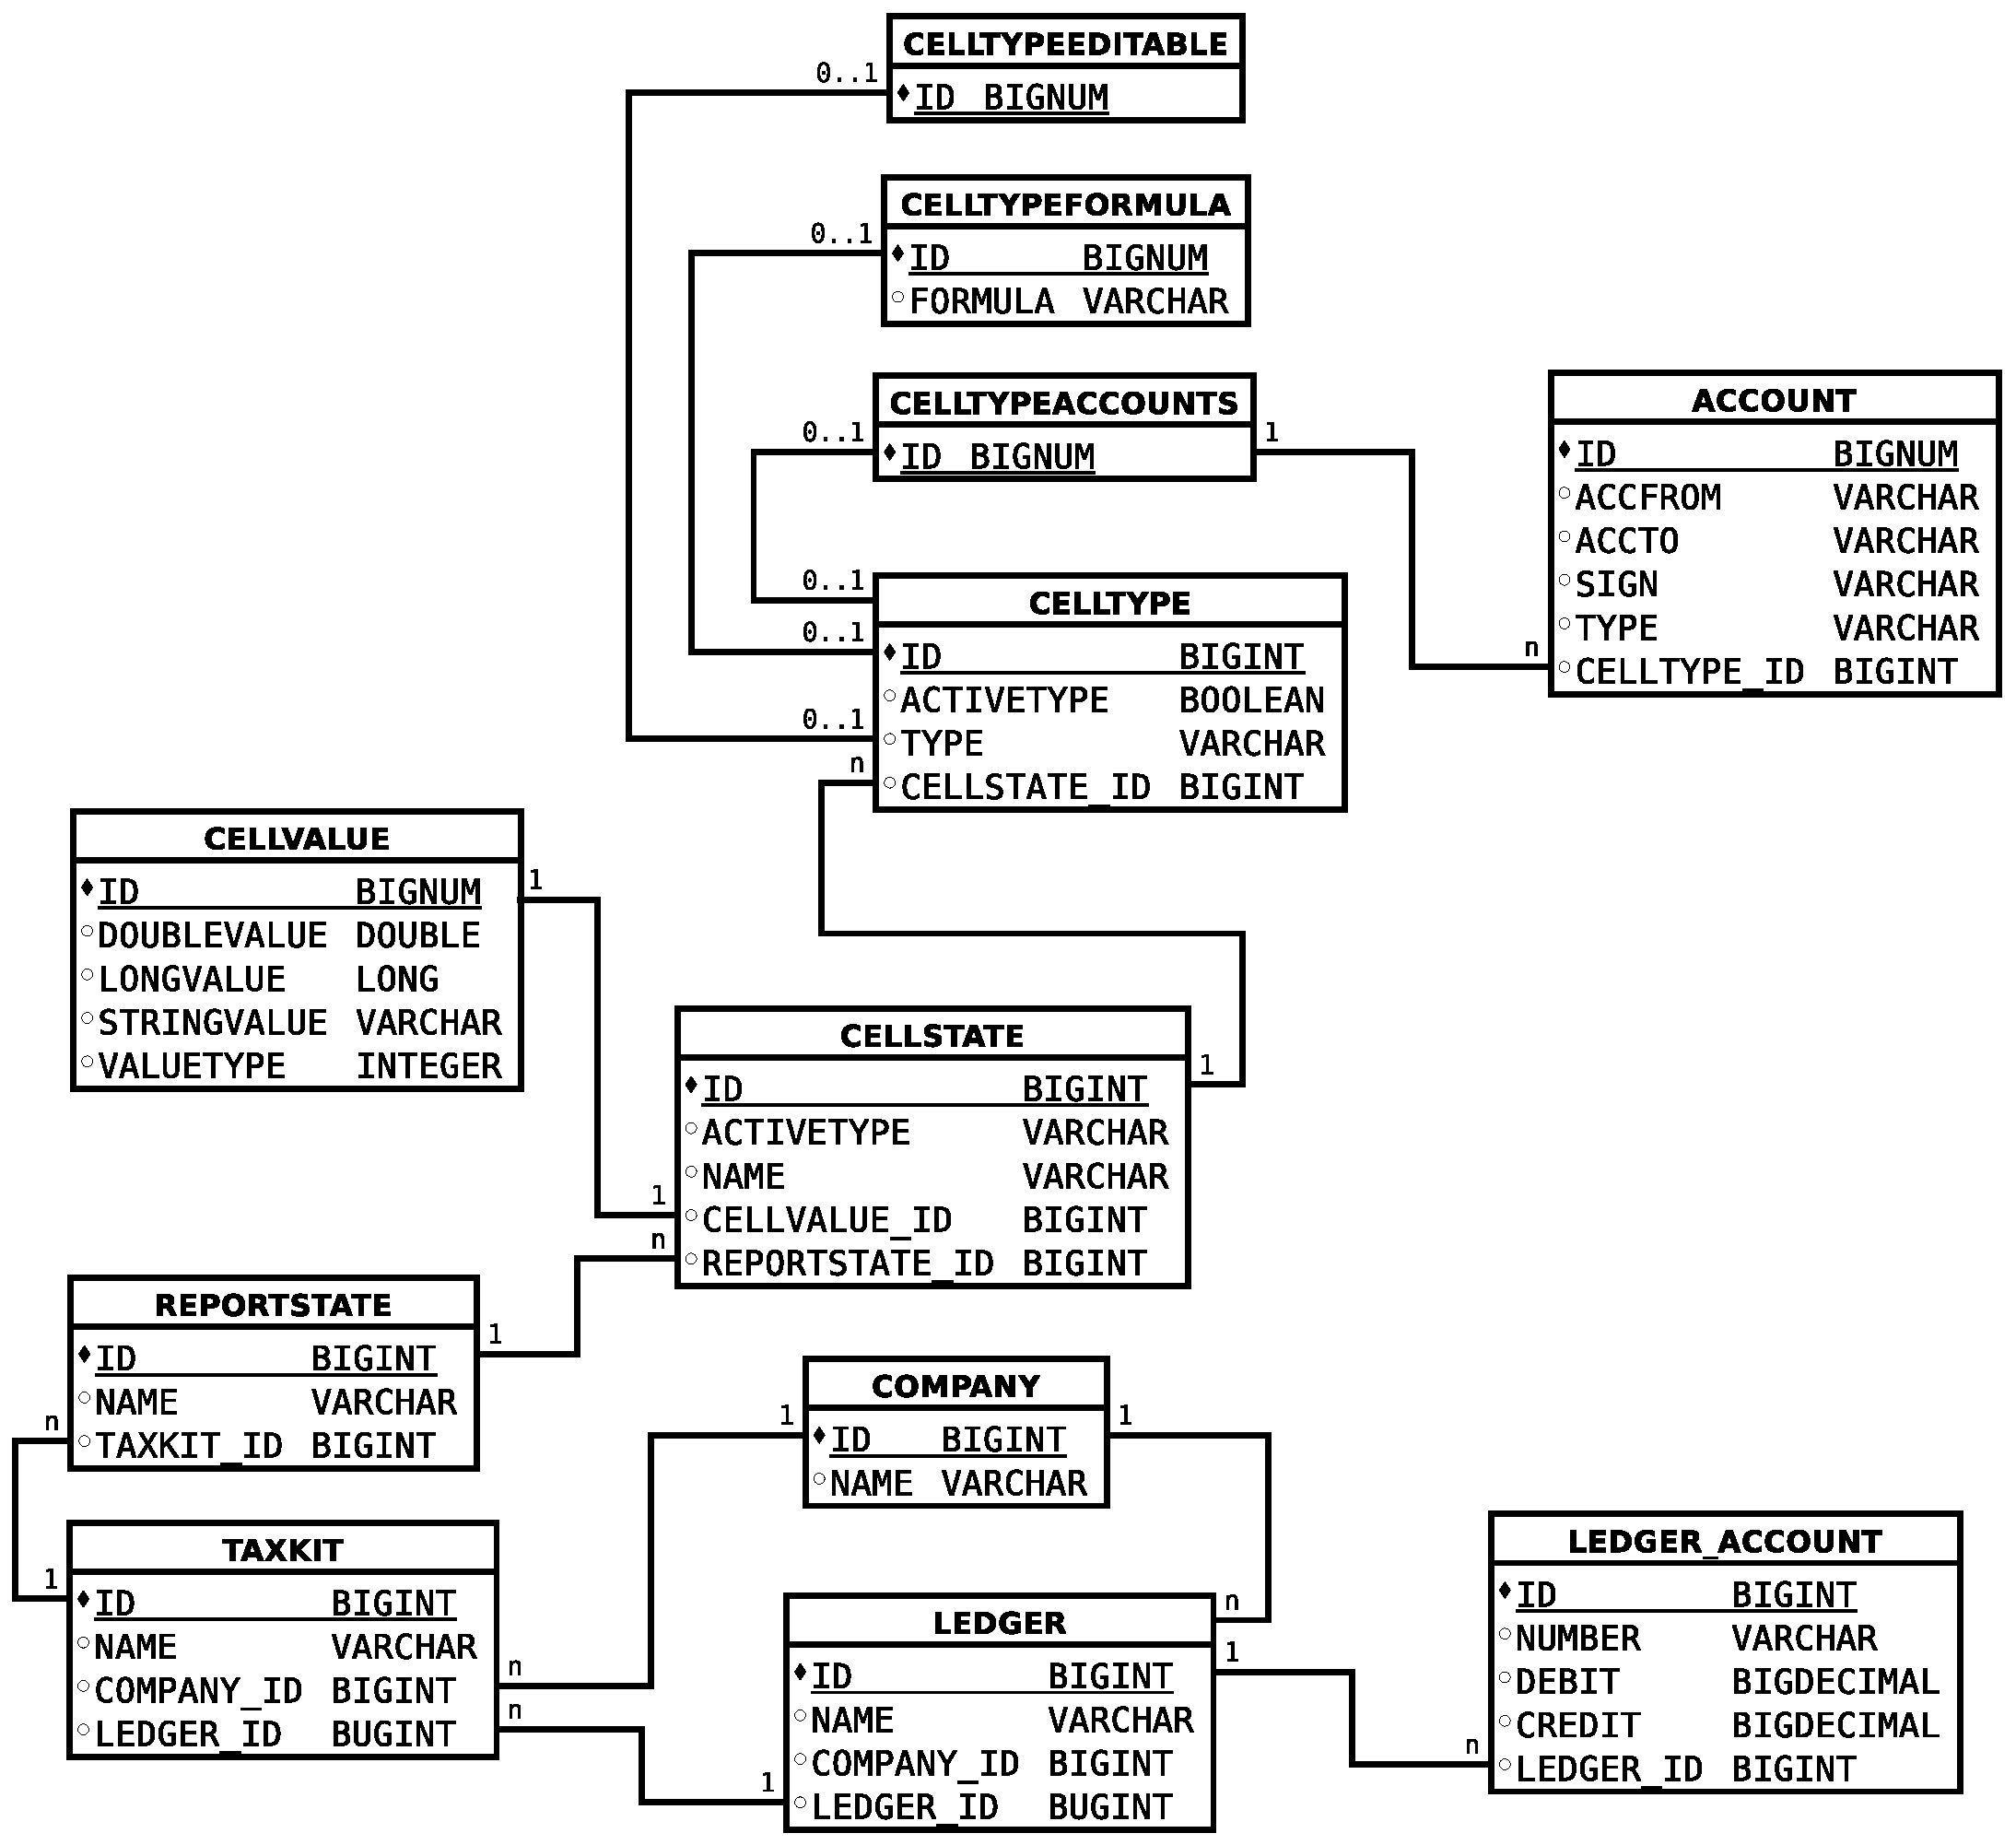
\includegraphics[scale=0.4]{uml/database}
%  \caption{Диаграмма базы данных}
%  \label{pic:database}
%\end{figure}
%\section{Тестирование}
В целях тестирования кода и контроля качества во время разработки были написаны модульные тесты. Тесты представляют собой набор утверждений, которые не должны быть опровергнуты в результате ожидаемой (корректной) работы тестируемого модуля. В данном контексте модулем является тестируемый класс. Наборы утверждений объединяются в методах. В рамках соглашения был использован следующий формат имени метода: ``testMethod'', где Method - название тестируемого метода.
Ниже приведен список классов, для которых были написаны модульные тесты:
\begin{itemize}
  \item XMLCellLoader
  \item XMLReportLoader
  \item ReportFactoryImpl
  \item ReportInterpreter
  \item ReportManager
  \item ReflectionAssembler
  \item XMLFileReader
  \item ReportStateController
  \item TaxKitReportStateDAOImpl
  \item ReportsServiceImpl
  \item (...)
\end{itemize}

(привести исходный код unit-тестов в приложении)

\chapter*{Охрана труда и экологическая безопасность}
\addcontentsline{toc}{chapter}{Охрана труда и экологическая безопасность}
(Обсепечение комфортных условий труда....)


\chapter*{Технико-экономическое обоснование}
\addcontentsline{toc}{chapter}{Технико-экономическое обоснование}
(Технико-экономическое обоснование системы учета и управления электронными налоговыми декларациями)


\begin{thebibliography}{99}
\addcontentsline{tok}{chapter}{Список литературы}

\bibitem{refwikidoc} Система автоматизации документооборота [Электронный ресурс] / Сообщество wikipedia, 2010. -- Режим доступа: http://ru.wikipedia.org/wiki/Система\_автоматизации\_документооборота -- Дата доступа 19.03.2010
\bibitem{refdoconline} Документооборот и делопроизводство. Системы электронного документооборота. [Электронный ресурс] . -- Режим доступа: http://www.doc-online.ru -- Дата доступа 19.03.2010
\bibitem{refwikixml} XML [Электронный ресурс] / Сообщество wikipedia, 2010. -- Режим доступа: http://ru.wikipedia.org/wiki/XML -- Дата доступа 19.03.2010
\bibitem{refspecxml} Extensible Markup Language (XML) 1.0 (Fifth Edition) [Электронный ресурс] / W3C. -- Режим доступа: Extensible Markup Language (XML) 1.0 (Fifth Edition) -- Дата доступа 19.03.2010
\bibitem{refelectrtaxesby} Государственная Целевая Программа по разработке программно-технического комплекса по автоматизации процесса расчета подлежащих уплате в бюджет сумм налогов, сборов (пошлин) и представлению в налоговые органы налоговых деклараций (расчетов) в электронном видена 2008 - 2010 годы [Электронный ресурс] : Аппарат Совета Министров Республики Беларусь. -- Режим доступа : http://www.government.by/ public/ shared/ rus/ solutions /rus\_solution101170\_1.pdf -- Дата доступа 19.03.2010
\bibitem{refwikitaxreturn} Налоговая декларация [Электронный ресурс] / Сообщество wikipedia, 2010. -- Режим доступа: http://ru.wikipedia.org/wiki/Налоговая\_декларация -- Дата доступа 19.03.2010

\end{thebibliography}

\end{document}
